%% 
%% Copyright 2019-2020 Elsevier Ltd
%% 
%% This file is part of the 'CAS Bundle'.
%% --------------------------------------
%% 
%% It may be distributed under the conditions of the LaTeX Project Public
%% License, either version 1.2 of this license or (at your option) any
%% later version.  The latest version of this license is in
%%    http://www.latex-project.org/lppl.txt
%% and version 1.2 or later is part of all distributions of LaTeX
%% version 1999/12/01 or later.
%% 
%% The list of all files belonging to the 'CAS Bundle' is
%% given in the file `manifest.txt'.
%% 
%% Template article for cas-sc documentclass for 
%% double column output.

%\documentclass[a4paper,fleqn,longmktitle]{cas-sc}
\documentclass[a4paper,fleqn]{cas-sc}

\usepackage[numbers]{natbib}
%\usepackage[authoryear]{natbib}
% \usepackage[authoryear,longnamesfirst]{natbib}
\usepackage[section]{placeins}
\usepackage{subcaption}
% \usepackage{subfig}
\usepackage{graphicx}
\usepackage{caption}

%%%Author definitions
\def\tsc#1{\csdef{#1}{\textsc{\lowercase{#1}}\xspace}}
\tsc{WGM}
\tsc{QE}
\tsc{EP}
\tsc{PMS}
\tsc{BEC}
\tsc{DE}
%%%

% Uncomment and use as if needed
%\newtheorem{theorem}{Theorem}
%\newtheorem{lemma}[theorem]{Lemma}
%\newdefinition{rmk}{Remark}
%\newproof{pf}{Proof}
%\newproof{pot}{Proof of Theorem \ref{thm}}
\newcommand{\etal}{\textit{et al.}}

\begin{document}
\let\WriteBookmarks\relax
\def\floatpagepagefraction{1}
\def\textpagefraction{.001}

% Short title
\shorttitle{Behavioural Analysis of Factors Influencing Online Food Ordering and Its Relation to Obesity}

% Short author
\shortauthors{S. M. Fazle Rabby Labib et~al.}

% Main title of the paper
\title [mode = title]{Behavioural Analysis of Factors Influencing Online Food Ordering and Its Relation to Obesity}                      
% Title footnote mark
% eg: \tnotemark[1]
% \tnotemark[1,2]

% Title footnote 1.
% eg: \tnotetext[1]{Title footnote text}
% \tnotetext[<tnote number>]{<tnote text>} 
% \tnotetext[1]{This document is the results of the research
%    project funded by the National Science Foundation.}

% \tnotetext[2]{The second title footnote which is a longer text matter
%    to fill through the whole text width and overflow into
%    another line in the footnotes area of the first page.}


% First author
%
% Options: Use if required
% eg: \author[1,3]{Author Name}[type=editor,
%       style=chinese,
%       auid=000,
%       bioid=1,
%       prefix=Sir,
%       orcid=0000-0000-0000-0000,
%       facebook=<facebook id>,
%       twitter=<twitter id>,
%       linkedin=<linkedin id>,
%       gplus=<gplus id>]
% \author[1,3]{CV Radhakrishnan}[type=editor,
%                         auid=000,bioid=1,
%                         prefix=Sir,
%                         role=Researcher,
%                         orcid=0000-0001-7511-2910]

% % Corresponding author indication
% \cormark[1]

% % Footnote of the first author
% \fnmark[1]

% % Email id of the first author
% \ead{cvr_1@tug.org.in}

% % URL of the first author
% \ead[url]{www.cvr.cc, cvr@sayahna.org}

% %  Credit authorship
% \credit{Conceptualization of this study, Methodology, Software}

% % Address/affiliation
% \affiliation[1]{organization={Elsevier B.V.},
%     addressline={Radarweg 29}, 
%     city={Amsterdam},
%     % citysep={}, % Uncomment if no comma needed between city and postcode
%     postcode={1043 NX}, 
%     % state={},
%     country={The Netherlands}}

% % Second author
% \author[2,4]{Han Theh Thanh}[style=chinese]

% % Third author
% \author[2,3]{CV Rajagopal}[%
%    role=Co-ordinator,
%    suffix=Jr,
%    ]
% \fnmark[2]
% \ead{cvr3@sayahna.org}
% \ead[URL]{www.sayahna.org}

% \credit{Data curation, Writing - Original draft preparation}

% % Address/affiliation
% \affiliation[2]{organization={Sayahna Foundation},
%     % addressline={}, 
%     city={Jagathy},
%     % citysep={}, % Uncomment if no comma needed between city and postcode
%     postcode={695014}, 
%     state={Trivandrum},
%     country={India}}

% % Fourth author
% \author%
% [1,3]
% {Rishi T.}
% \cormark[2]
% \fnmark[1,3]
% \ead{rishi@stmdocs.in}
% \ead[URL]{www.stmdocs.in}

% \affiliation[3]{organization={STM Document Engineering Pvt Ltd.},
%     addressline={Mepukada}, 
%     city={Malayinkil},
%     % citysep={}, % Uncomment if no comma needed between city and postcode
%     postcode={695571}, 
%     state={Trivandrum},
%     country={India}}

% % Corresponding author text
% \cortext[cor1]{Corresponding author}
% \cortext[cor2]{Principal corresponding author}

\author[1]{S. M. Fazle Rabby Labib}[prefix= , type= editor,
orcid=0009-0008-5397-3881]

% Corresponding author indication
\cormark[1]

% % Footnote of the first author
% \fnmark[1]

% Email id of the first author
\ead{s.m.fazle.rabby.labib@g.bracu.ac.bd}

% URL of the first author
\ead[url]{www.bracu.ac.bd}

%  Credit authorship
\credit{Conceptualization, Formal Analysis, Investigation, Methodology, Software Visualization, Writing - original draft}



% Second author
\author[1]{Fahmida Zaman Achol}[prefix= , orcid = 0009-0001-6119-2179]

% Email id of the Second author
\ead{fahmida.zaman.achol@g.bracu.ac.bd}

% URL of the Second author
\ead[url]{www.bracu.ac.bd}

\credit{Conceptualization, Formal Analysis, Investigation, Methodology, Visualization, Writing - original draft}

% Third author
% \author[1]{Md. Aqib Jawwad}[%
%    % role=Co-ordinator,
%    % suffix=Jr,
%    ]
\author[1]{Md. Aqib Jawwad}[prefix= , orcid = 0009-0001-0043-5798]
% % \fnmark[2]
\ead{md.aqib.jawwad@g.bracu.ac.bd}
\ead[URL]{www.bracu.ac.bd}

\credit{Conceptualization, Formal Analysis, Investigation, Methodology, Writing - original draft}

% Fourth author
\author[1]{Md. Golam Rabiul Alam}[prefix= Dr., orcid = 0000-0002-9054-7557]
% \cormark[2]
% \fnmark[1,3]
\ead{rabiul.alam@bracu.ac.bd}
\ead[URL]{www.bracu.ac.bd}
\credit{Conceptualization, Methodology, Project administration, Resources, Supervision, Writing – review \& editing}

% Sixth author
\author[3]{Md Iftekharul Mobin}[prefix= Dr., orcid = 0000-0002-3065-2486]
% \cormark[2]
% \fnmark[1,3]
\ead{iftekhar.mobin@aiub.edu}
\ead[URL]{www.aiub.edu}
\credit{Supervision, Writing – review \& editing}

% Fifth author
\author[2]{Ashis Talukder}[prefix= Dr., orcid = 0000-0003-2991-9136]
% \cormark[2]
% \fnmark[1,3]
\ead{ashis@du.ac.bd}
\ead[URL]{www.du.ac.bd}
\credit{Supervision \& Funding acquisition}

% Address/affiliation
\affiliation[1]{organization={BRAC University},
    addressline={Kha 224 Bir Uttam Rafiqul Islam Avenue, Merul Badda}, 
    city={Dhaka},
    citysep={}, % Uncomment if no comma needed between city and postcode
    postcode={1212}, 
    % state={},
    country={Bangladesh}}
    
% Address/affiliation
\affiliation[2]{organization={University of Dhaka},
    addressline={Nilkhet Rd}, 
    city={Dhaka},
    citysep={}, % Uncomment if no comma needed between city and postcode
    postcode={1000}, 
    % state={},
    country={Bangladesh}}

% Address/affiliation
\affiliation[3]{organization={American International University Bangladesh},
    addressline={Kuratoli.}, 
    city={Dhaka},
    citysep={}, % Uncomment if no comma needed between city and postcode
    postcode={1229}, 
    % state={},
    country={Bangladesh}}
    
% Corresponding author text
\cortext[cor1]{Corresponding author: S. M. Fazle Rabby Labib, Phone: +880 1623925656. Department of Computer Science \& Engineering, Brac University, Kha 224 Bir Uttam Rafiqul Islam Avenue, Merul Badda, Dhaka 1212, Bangladesh}

% Footnote text
% \fntext[fn1]{This is the first author footnote. but is common to third
%   author as well.}
% \fntext[fn2]{Another author footnote, this is a very long footnote and
%   it should be a really long footnote. But this footnote is not yet
%   sufficiently long enough to make two lines of footnote text.}

% % For a title note without a number/mark
% \nonumnote{This note has no numbers. In this work we demonstrate $a_b$
%   the formation Y\_1 of a new type of polariton on the interface
%   between a cuprous oxide slab and a polystyrene micro-sphere placed
%   on the slab.
%   }

% Here goes the abstract
\begin{abstract}
% This template helps you to create a properly formatted \LaTeX\ manuscript.
% 
% \noindent\texttt{\textbackslash begin{abstract}} \dots 
% \texttt{\textbackslash end{abstract}} and
% \verb+\begin{keyword}+ \verb+...+ \verb+\end{keyword}+ 
% which
% contain the abstract and keywords respectively. 
% 
% \noindent Each keyword shall be separated by a \verb+\sep+ command.
% The purpose of this research is to determine what influences people to order food online and the intensity of ordering as well as to see if there is any correlation between online food ordering and obesity among the people of Bangladesh. We conduct an online questionnaire survey analyzing data from 343 participants aged 16-30 residing in Bangladesh. We use Ordinary Least Squares, Decision Tree, and Random Forest to determine the factors influencing customers' decision to order food online. The most influential factors are impulsive decision (OLS coefficient = 0.90), convenience of ordering (OLS coefficient = 0.65), variety of options available (OLS coefficient = 0.15), and promotional offers and discounts (OLS coefficient = 0.33). Then, we conduct statistical analyses to determine the correlation between obesity and the intensity of online food ordering. We find a weak positive relationship (p-value = $2.43^{-7}$, coefficient = 0.28). We classify frequent users of OFO by using classifiers such as Logistic Regression, Naive Bayes, Decision Tree Classifier, Random Forest Classifier, Gradient Boosting Machine and K-Nearest Neighbors, where we find Random Forest to perform the best with an accuracy of 81\%. Customer segmentation using K-Means clustering reveals that infrequent orders perceive OFO services as expensive, while frequent customers find the food lacking in nutrition. Several Chi-Squared Tests are conducted, revealing significant associations. Firstly, tech savviness is strongly related to perception of OFO services as user-friendly (p $<$ 0.001). Secondly, individuals leading busy lives tend to make impulsive decisions (p $<$ 0.001). Lastly, affordability of OFO services correlates with ordering behavior driven by promotional offers and discounts (p $<$ 0.001). These insights, along with the developed prediction models and customer segmentation, contribute to a deeper understanding of consumer behaviour in an increasingly digitalized food landscape.
%The purpose of this research is to determine what influences people to order food online (OFO) services and the intensity of ordering as well as to see if there exists any correlation between online food ordering and obesity among the people of Bangladesh. We conduct an online questionnaire survey analyzing data from 343 participants aged 16-30 residing in Bangladesh. We use Ordinary Least Squares, Decision Tree, and Random Forest to determine the factors influencing customers' decision to order food online. The most influential factors are impulsive decisions, convenience of ordering, variety of options available, and promotional offers and discounts. Then, we conduct statistical analyses to determine the correlation between obesity and the intensity of online food ordering. We find a weak positive relationship (p-value = $2.43^{-7}$, coefficient = 0.28). We classify frequent users of OFO by using classifiers such as Logistic Regression, Naive Bayes, Decision Tree Classifier, Random Forest Classifier, Gradient Boosting Machine and K-Nearest Neighbors, where we find Random Forest to perform the best with an accuracy of 81\%. Customer segmentation using K-Means clustering reveals that people who order food rarely, tend to consider OFO services to be expensive. Whereas frequent customers find the ordered food to lack proper nutritional values. Several Chi-Squared Tests are conducted, revealing significant associations. Firstly, tech savviness is strongly related to the perception of OFO services as user-friendly. Secondly, individuals leading busy lives tend to make impulsive decisions. Lastly, the affordability of OFO services correlates with ordering behavior driven by promotional offers and discounts. These insights, along with the developed prediction models and customer segmentation, contribute to a deeper understanding of consumer behaviour in an increasingly digitalized food landscape.
This research endeavors to unravel the determinants shaping individuals' decisions to engage with online food ordering (OFO) services and the subsequent intensity of their ordering habits. Additionally, it explores whether a correlation exists between OFO and obesity, encompassing diverse consumer demographics. Drawing insights from an online questionnaire survey with 343 participants aged 16–30, our study employs a multifaceted approach, incorporating Ordinary Least Squares, Decision Tree, and Random Forest methodologies. The identified influential factors span impulsive decision-making, ordering convenience, variety of options, and the allure of promotional offers and discounts. Statistical analyses reveal nuanced patterns, indicating a weak positive relationship between obesity and the frequency of online food ordering (p-value = $2.43^{-7}$, coefficient = 0.28). To analyze consumer behavior, our study utilizes diverse classifiers such as Logistic Regression, Naive Bayes, Decision Tree Classifier, Random Forest Classifier, Gradient Boosting Machine, and K-Nearest Neighbors. Notably, Random Forest emerges as a robust classifier, achieving an accuracy of 81\% in classifying frequent users of OFO. Customer segmentation through K-Means clustering uncovers varied preferences. Users with infrequent OFO habits often perceive the services as expensive, while frequent users express concerns about the nutritional content of the ordered food. Chi-squared tests highlight significant associations, indicating that tech savvy correlates with the perception of OFO services as user-friendly. Moreover, globally, individuals leading hectic lifestyles often exhibit impulsive decision-making tendencies, with the affordability of online food ordering (OFO) services closely tied to ordering behavior shaped by promotional offers and discounts. These findings, accompanied by developed prediction models and a customer segmentation approach, contribute valuable insights to the understanding of universal consumer behavior in an ever-evolving, digitalized food landscape.

\end{abstract}

% Use if graphical abstract is present
% \begin{graphicalabstract}
% \includegraphics{figs/grabs.pdf}
% \end{graphicalabstract}

% Research highlights
% \begin{highlights}
% \item Research highlights item 1
% \item Research highlights item 2
% \item Research highlights item 3
% \end{highlights}

% Keywords
% Each keyword is separated by \sep
\begin{keywords}
Online Food Ordering \sep Obesity \sep Behavioural Analysis \sep Machine Learning \sep Customer Segmentation \sep Hypothesis Testing
% \sep Factor Analysis
\end{keywords}


\maketitle

\section{Introduction}
% The Elsevier cas-sc class is based on the
% standard article class and supports almost all of the functionality of
% that class. In addition, it features commands and options to format the
% \begin{itemize} \item document style \item baselineskip \item front
% matter \item keywords and MSC codes \item theorems, definitions and
% proofs \item labels of enumerations \item citation style and labelling.
% \end{itemize}
% 
% This class depends on the following packages
% for its proper functioning:
% 
% \begin{enumerate}
% \itemsep=0pt
% \item {natbib.sty} for citation processing;
% \item {geometry.sty} for margin settings;
% \item {fleqn.clo} for left aligned equations;
% \item {graphicx.sty} for graphics inclusion;
% \item {hyperref.sty} optional packages if hyperlinking is
%   required in the document;
% \end{enumerate}  
% 
% All the above packages are part of any
% standard \LaTeX{} installation.
% Therefore, the users need not be
% bothered about downloading any extra packages.

% Online Food Ordering (OFO) Services are making our life easier but due to most food consisting of saturated fat, salt and sugar, we are also seeing an increase in major health issues like high blood pressure, obesity, diabetes, cardiovascular diseases and even several types of cancer. Overweight and Obesity is one of the most common and concerning causes of food ordering and it is increasing at an alarming rate every year. The proportion of overweight and obesity among adults is rising in developed as well as developing countries, notably among young adults. The World Health Organization (WHO) defines obesity as an abnormal accumulation of fat in the body that harms one's health. It is a worldwide public health problem which is increasing rapidly as the rate of obesity has tripled since 1975~\cite{WHO_Obesity_Factsheet}. Obesity is determined by measuring the Body Mass Index (BMI), which is the ratio of a person's weight in kilograms to their height in meters. OFO is currently at its peak because of the accessibility and faster services, which raises the question of its relation to obesity. Although, there exist few papers on what influences a user's decision to order food online, nearly no research has been done on what encourages people to order frequently. We aim to fill that gap. Our purpose here is to find the factors that cause people to use online food ordering services and if the ordering frequency plays any part in causing obesity.

% % \subsection{Research Problem}
% With the increase in the popularity of delivered goods, the food sector has seen a major boom as well. Especially during the time of COVID-19, when people had no choice but to resort to online food ordering services for the sake of their safety and convenience. What once was a physical trip to the restaurant, now can easily be done with just a few clicks on our phones. According to 2022 research by Allied Market Research~\cite{amr_food_delivery_app_statistics}, in 2020, the worldwide market for mobile food delivery apps was valued at \$6,752.32 million. This rise in popularity can be seen in Bangladesh too as online food delivery services like foodpanda, HungryNaki and Pathao Food are getting popular all over the country. Yet, it is still unknown what factors are influencing people to order food online. It could be to save time or to save money and order something with discounts. 
% % Maybe it is because of how convenient it is to order food online or maybe it is driven by the hedonic motivation to eat comfort food. 

% Along with the popularity of online food ordering services, there has been an increase in obesity rates among adults. According to WHO’s World Obesity Day 2022 study~\cite{who_world_obesity_day_2022}, more than 1 billion people worldwide are obese and this number is still increasing. This rise might have some relation to the increase in online food ordering. According to National Health Service (NHS)~\cite{nhs_obesity_causes}, obesity is the result of consuming excessive amounts of food and not engaging in enough physical activity. When large quantities of calories, particularly from saturated fat, salt, and sugar, are consumed but not used through exercise or physical activity, the excess energy is stored as fat in the body. Excess amounts of fat will lead to obesity. Most of the online food ordering services are offering restaurants that sell food that is highly processed, and filled with large amounts of saturated fat, sugar and salt. Along with that none of these apps provide any sort of nutritional information about the foods that are being ordered.

% As the rate of obesity increases, it is now considered a global epidemic. According to a 2016 study by Hruby et al.~\cite{hruby_determinants_2016}, being obese can lead to serious health issues such as stroke, heart disease, type 2 diabetes, specific types of cancer, and early death. Therefore, it has become severely important to figure out what factors are causing it so that we can take measures to stop it. 

% In order to do that we need a significant amount of data which will be analyzed over the course of a few months. A problem arises as there is little to no data available related to this problem worldwide let alone in Bangladesh. As a result, the research is trying to address the following questions: 

% \hfill \break
% \textbf{\emph{What factors are influencing users’ decision to order food through online services and if the intensity of ordering has any correlation with the increase in obesity rates among people of Bangladesh? To see if there exists any relationship between the factors. Moreover, to see if the users can be classified as well as segmented into multiple clusters.}}

% % \subsection{Research Contributions}

% In this research, we created a dataset on Bangladeshi customers using OFO services. We find the factors that influence the use of OFO services. We try to see if there exists any correlation between BMI and orders per month. Moreover, we develop a prediction model that classifies frequent online food orders. We apply customer segmentation to divide the user base in two clusters and analyze the results. Finally we do some hypothesis testing to find relation between the factors. This kind of research is non existent in Bangladeshi context  The main contributions are summarized as follows:

% \begin{enumerate}

%     \item We have identified the factors that influence people to order food online. To do this we used the feature importance of Decision Tree and Random Forest, we also have used the coefficient values of Ordinary Least Squares.
    
%     \item We did some hypothesis testing among the factors to determine relation between each other. This is done by using Chi-squared test of independence.
    
%     \item We have found that even though it is very weak, but there exists correlation between obesity and orders per month. We also conducted correlation analysis between other BMI categories and orders per month as well as between physical activity, order history and orders per month. For this, we used Pearson Correlation, Spearman's Rank Correlation and Point Bi-serial Correlation. 

%     \item We have developed a model that successfully classifies frequent users of OFO services. We use several classifiers such as Logistic Regression, Naive Bayes, Decision Tree, Random Forest, Gradient Boosting Machine and K-Nearest Neighbors.

%     \item We apply customer segmentation on our data and divide the users into two clusters, analyze the data and show our findings. This is done using K-Means. Moreover, we use PCA to do some dimensionality reduction.

%     \item We create a dataset of Bangladeshi OFO service users which we consider to be an important contribution since this type of dataset is non existent specially in Bangladeshi context.

% \end{enumerate}

% Online Food Ordering (OFO) Services have transformed our access to meals, offering convenience unparalleled by traditional dining. However, this convenience comes with health concerns, notably the rise in major health issues like high blood pressure, obesity, diabetes, cardiovascular diseases, and various types of cancer. Obesity, in particular, has become a critical global health challenge. It is attributed to an abnormal accumulation of body fat that significantly impacts overall health and well-being. The WHO~\cite{WHO_Obesity_Factsheet} reports a tripling of obesity rates since 1975, marking it a pressing public health problem worldwide. The surge in OFO services has particularly amplified during COVID-19, redefining how we procure meals. With market values skyrocketing globally, including within Bangladesh, platforms like foodpanda, HungryNaki, and Pathao Food have become integral parts of modern food consumption. Yet, what influences individuals to use these services and how this behaviour might relate to the rise in obesity remains largely unexplored.

% The linkage between the popularity of OFO services and the escalating rates of obesity is a pressing concern. According to the National Health Service (NHS)~\cite{nhs_obesity_causes} obesity stems from excessive calorie intake and insufficient physical activity. Most OFO platforms offer highly processed, calorie-rich food options, lacking vital nutritional information, potentially contributing to this concerning trend.

% Our research aims to bridge this gap by investigating the factors influencing OFO service usage and its potential correlation with rising obesity rates, particularly among the Bangladeshi populace. To do that we need a significant amount of data. A problem arises as there is little to no data available related to this problem worldwide let alone in Bangladesh. As a result, the research is addressing the following questions: 

Online Food Ordering (OFO) Services have globally transformed meal accessibility, offering unparalleled convenience compared to traditional dining. However, this convenience raises health concerns, contributing to major issues such as high blood pressure, obesity, diabetes, cardiovascular diseases and various types of cancer. The World Health Organization (WHO)~\cite{WHO_Obesity_Factsheet} notes a tripling of obesity rates since 1975, emphasizing its urgency as a global public health problem. During the COVID-19 pandemic, the surge in OFO services has redefined how we procure meals globally, including in Bangladesh. Platforms like foodpanda, HungryNaki, and Pathao Food have become integral to modern food consumption. Despite their widespread use, the factors~\cite{dakin2024can} influencing individuals to adopt these services and their potential contribution to the global rise in obesity~\cite{weydmann2023overweight} remain largely unexplored.

Bangladesh, as a valuable test case, provides insights into how OFO services impact diverse cultural and geographical contexts. Understanding these dynamics on a global scale is essential for devising effective strategies to address health implications associated with the widespread adoption of online food ordering services.

The linkage between the widespread popularity of Online Food Ordering (OFO) services and the rising prevalence of obesity raises significant concerns. According to the National Health Service (NHS)~\cite{nhs_obesity_causes}, obesity is attributed to excessive calorie intake and inadequate physical activity. OFO platforms, often offering highly processed, calorie-rich food options with limited nutritional information, may contribute to this severe trend.

This research aims to address this knowledge gap by investigating the factors influencing OFO service usage and its potential correlation with the increasing rates of obesity. Our qualitative survey concentrates on the Bangladeshi population, serving as a case study scenario. The difficulty arises from the limited availability of comprehensive data on this matter, both on a global scale and specifically within Bangladesh. Thus, this research aims to address the following questions: 

% \textbf{\emph{What factors influence users' decisions to order food through online services, and does the intensity of ordering correlate with the increase in obesity rates among the people of Bangladesh? Is there a relationship between these factors? Additionally, can users be effectively classified and segmented into multiple clusters based on their behaviour?}}

\begin{enumerate}

    \item What factors influence users' decisions to order food through online services?
    
    \item Does the intensity of ordering correlate with the increase in obesity rates %among the people of Bangladesh?

    \item Does the intensity of ordering correlate with the increase in obesity rates %among the people of Bangladesh?

    \item Can users be effectively classified and segmented into multiple clusters based on their behaviour?
    

\end{enumerate}

Within the framework of this research, we curate a pioneering dataset focusing on Bangladeshi customers engaging with Online Food Ordering (OFO) services. Our objective is to explore the determinants influencing the adoption of OFO services and investigate potential correlations between Body Mass Index (BMI) and monthly order frequencies. Additionally, we craft a predictive model designed to classify users exhibiting frequent online food ordering behaviors~\cite{screti2024understanding}. Applying advanced customer segmentation techniques, we categorize the user base into two distinct clusters, facilitating a detailed and nuanced analysis. To further deepen our insights, we undertake hypothesis testing to unveil relationships between various factors. Its primary contributions can be summarized as follows:

\begin{enumerate}

    \item We identify the factors driving the adoption of OFO services among Bangladeshi consumers, utilizing techniques such as Decision Tree, Random Forest, and Ordinary Least Squares to assess feature importance.
    
    \item We conduct hypothesis testing to determine the relation among influencing factors using the Chi-squared test of independence.
    
    \item We have found that even though it is very weak, there exists a correlation between obesity and orders per month. We also conducted a correlation analysis between other BMI categories and orders per month as well as between physical activity, order history, and orders per month. For this, we used Pearson Correlation, Spearman's Rank Correlation, and Point Bi-serial Correlation.  
    
    We explore the correlation, albeit weak, between BMI and monthly order frequencies using various correlation analyses such as Pearson, Spearman's Rank, and Point Bi-serial correlations. Additionally, we examine the correlations among BMI categories, physical activity, order history, and order frequencies.

    \item We develop a model to classify frequent users of OFO services, employing classifiers such as Logistic Regression, Naive Bayes, Decision Tree, Random Forest, Gradient Boosting Machine, and K-Nearest Neighbors.

    \item We apply customer segmentation techniques, specifically K-Means, and PCA, to find user clusters, offering insights into consumer behaviour.

    \item We create a novel dataset of Bangladeshi OFO service users, a significant addition to the Bangladeshi research landscape.

\end{enumerate}


% \subsection{Research Organization}
% The rest of the paper is organized in the following order: 

% In section 2, we provide some literature review. It contains how previous researches were conducted and their findings. In section 3, we provide the methodology behind our work. In section 4, we show our findings and finally, in section 5, we wrap up by sharing some concluding remarks, acknowledging the limitations and the scope for future work.

\section{Literature Review}

% Online food ordering has become popular lately, which brings us to the question of what influences people to order food through online platforms. 

% The following 2020 paper by Kale et al.~\cite{kale_customer_perception_2020}, the authors describe the customer perception regarding OFO alongside its significance. The authors stated that although online food ordering services are vast and diverse, based on the data and research, it is shown that 50\% of people prefer online food delivery services instead of going out because of the convenience and flexibility. Additionally, ease of payment, sales promotions, and diverse reviews from different platforms play a crucial role in more consumers changing their perception about online food ordering.

% Alagoz et al.~\cite{alagoz_2012} in their, propose an analysis based on customer attitudes in terms of ordering food using the internet among Turkey's university students using the Technology Acceptance Model (TAM). The hypothesis of this research work mentions that the easy online ordering process encourages students to choose the online food ordering system. Cronbach's alpha coefficient is used and considered with satisfactory value.

% % In this 2022 study by Jahidi et al.~\cite{jahidi_2022}, the positivist approach is applied to find factors that affect the attitude towards online food retailing by involving respondents who often use online food ordering systems in Bandung, Indonesia. Questionnaires are used to collect data. They stated by mentioning that a larger sample would have given a better representation of the population and the motivations may vary across other nations because of differences in culture and the acceptance of technological advancements.

% The authors of this 2020 research~\cite{parameshwaran_2020}, study the factors that influence online consumers behaviour in Salem, Tamil Nadu. After analysis, they find some statistical information such as how most respondents are females and most online shoppers are below age 30. They also find most online shoppers are influenced by online advertisements or through their friends. The authors conclude that the most important factor for online shopping is saving time and transportation costs.

% Some of the research included the changes that come to decision-making when there is a global pandemic like COVID-19. 

% This research~\cite{anam_2021}, shows the factors that are increasing online shopping during the pandemic period and how social distancing has brought a lot of change in consumer behaviour over the two years. The aim is to detect consumers adopting and exploring different platforms and payment systems over the years and how it pushes people to access things more online. 

% The writers of this article~\cite{inthong_2022}, explain how individuals act when using OFO platforms, particularly during the COVID-19 epidemic. The urge to use the OFO app for ordering food online is strongly influenced by mindset, personal standards, as well as perceived behavioural control. This study's sole drawback is the necessity to test a wide range of delivery applications in order to analyze user behaviour and measure people's opinions on food delivery services. Users' preferences may differ from nation to country or even from area. 

% This study~\cite{hong_2021}, looks at how customers' intentions to use online food delivery services are affected before and during the COVID-19 pandemic. The results show that factors such as Perceived Ease of Use, Perceived Usefulness Trust, Price Saving Benefits, Time Saving Benefits, Perceived Severity, and Perceived Vulnerability have a positive influence on customers' intentions to use OFO services. However, the study finds that customers are more likely to adopt online food delivery applications if they find them useful. 

% With the rise of obesity around the world, it is important to study what risks this medical condition brings to our daily lives. 

% Chatterjee et al~\cite{chatterjee_2020}. with their 2020 study, try to identify risk factors connected with obesity and overweight with a machine learning approach. The primary goal of this study is not to highlight any risk predicting model but to review several machine learning methods and execution using health data. An epidemiological study shows how several groups of people's lifestyles lead to illness, its reason and its risks. Chatterjee et al. find the riskiest factors of obesity through selected literature studies. Using statistical, machine learning and data visualization methods, potential risk factors have been identified by the authors. Here, the authors focus on designing, testing, evaluating and developing the eCoach system to achieve the goal. 

% In their 2003 paper~\cite{prentice_2003}, Prentice and colleagues review a number of studies on the energy density of food and its impact on energy consumption. By analyzing popular fast food websites, the authors find that many fast food items have a high energy density, with an average energy density that is 65\% higher than the British average diet and two times higher than preferred healthy diets. This can lead to weight gain and obesity. The authors identify factors such as eating diversity, inactive lifestyle, and environmental changes as contributing to obesity. They propose that energy density plays a key role in this process. Children are particularly at risk due to their undeveloped cognitive dietary restraints. 

% In his research, Dave et al.~\cite{dave_2009}, represents the relationship between adults' fast food consumption frequency and their attitude towards it throughout their article. This study primarily uses telephone surveys as a cross-sectional examination to assess people's eating habits and opinions. The target of the study is to represent the unhealthy perspective of fast foods and to reduce their consumption. 

% This research~\cite{ayubi_2021}, examines the factors that influence the frequency of online food ordering for high-risk food. The study finds that young adults are influenced by social, environmental, and appealing advertisements, which leads to consuming food through online food ordering services. While the study emphasizes the case that encouraging positive influences could be advantageous even when the link between cause and effect has not been determined. 

% The author here~\cite{harahap_2020} examines the relationship between the type and frequency of online food ordering and obesity among university students. They also note that online fast food can contribute to obesity, as it is affordable, convenient and appealing to current tastes, leading to over consumption. Women are more likely to order food online, but the portions are not large enough to be considered a full meal. Additionally, a lack of physical activity among this group can also contribute to obesity over time. 

% In this paper~\cite{kurniawati_2021}, the authors try to correlate online food ordering and nutritional status. They use descriptive correlation with a cross-sectional approach and study 388 college students in Surabaya, Indonesia. The majority of the ordered meal is high in calories, fat, sodium, and unsaturated sugar according to the analysis of all the data. There is no connection between OFO and the nutritional state of college students. 

% In summary, we can see that recent studies related to this issue mostly talk about online shopping as a whole or only study customer behaviour in order to grow the OFO industry even more. The studies that have correlated the intensity of buying food through online mediums and obesity are mostly based in other countries. On top of that the datasets used on those researches are not available for future works. None of the studies have been specifically done with the people of Bangladesh. With our research, we want to tackle the issues from the Bangladeshi perspective.

The surge in online food ordering (OFO) has reshaped consumer habits, which brings us to explore its multifaceted impact. Here, we examine various studies related to OFO, encompassing its influence on consumer behaviour, health implications like obesity, and the factors driving its popularity.

Kale \etal~\cite{kale_customer_perception_2020} highlight convenience and flexibility as prime reasons behind the preference for using OFO which is supported by Alagoz \etal~\cite{alagoz_2012} who emphasize the significance of an easy ordering process, particularly among university students. Similar results can be found in the study conducted by Vinish \etal~\cite{vinish2021} which indicates convenience of placing orders, the quality and availability of food, restaurant reviews, offers and discounts, quick delivery, and a wide choice of restaurants are crucial for customer satisfaction. On the other hand, Parameshwaran \etal~\cite{parameshwaran_2020} and Anam \etal~\cite{anam_2021} delve into the influence of advertising, social factors, and the shift to online platforms, accentuated during the COVID-19 pandemic.

In examining health ramifications, Chatterjee \etal~\cite{chatterjee_2020} use machine learning methods to explore obesity risk factors. They emphasize the need to understand the lifestyle choices of consumers. Prentice \etal~\cite{prentice_2003} shed light on the role of energy-dense food in obesity, stressing its prevalence in fast food offerings and its adverse impact, especially among children. Meanwhile, studies by Harahap \etal~\cite{harahap_2020} and Kurniawati \etal~\cite{kurniawati_2021} emphasize the correlation between online food ordering, dietary choices, and obesity risks among university students, offering insights into nutritional aspects and consumption patterns, albeit with differing conclusions. Whereas Harahap \etal suggest OFO and fast food consumption lead to overconsumption which contributes to obesity, Kurniawati's study reveals the nutritional content of the meals ordered online does not establish a direct link between OFO and the nutritional state of college students. This study by Dana \etal~\cite{dana2021} highlights that younger users with higher BMI tend to use OFO services.

Studies conducted by Hong \etal~\cite{hong_2021} and Ayubi \etal~\cite{ayubi_2021} analyze customer intentions, behavioural aspects, and influences across demographics and regions. Similarly, Jahidi \etal~\cite{jahidi_2022} and Inthong \etal~\cite{inthong_2022} concur, highlighting the potential variation in motivations across different regions.

Despite extensive research, gaps persist, particularly regarding the Bangladeshi perspective. Existing studies primarily hail from diverse geographical locations, with datasets unavailable for future research. This gap underscores the need for localized studies in Bangladesh to understand cultural nuances and their influence on OFO dynamics. In contrast to prior methodologies employing behavioural intention models like TAM~\cite{tam} and UTAUT~\cite{utaut} for data analysis, our approach leverages machine learning techniques.

In summary, while existing studies provide invaluable insights into OFO's global impact, there's a clear need for localized research in Bangladesh. Understanding how OFO affects Bangladeshi consumers, considering cultural, socioeconomic, and dietary differences, will be crucial for informing policies and practices in this evolving landscape.

\section{Methodology}
% In this section, we talk about the the procedure of collecting data and the methodologies behind our experiments.
% In this section, we discuss the detailed methodology of our research work.

\begin{figure}[htb]
  \centering
  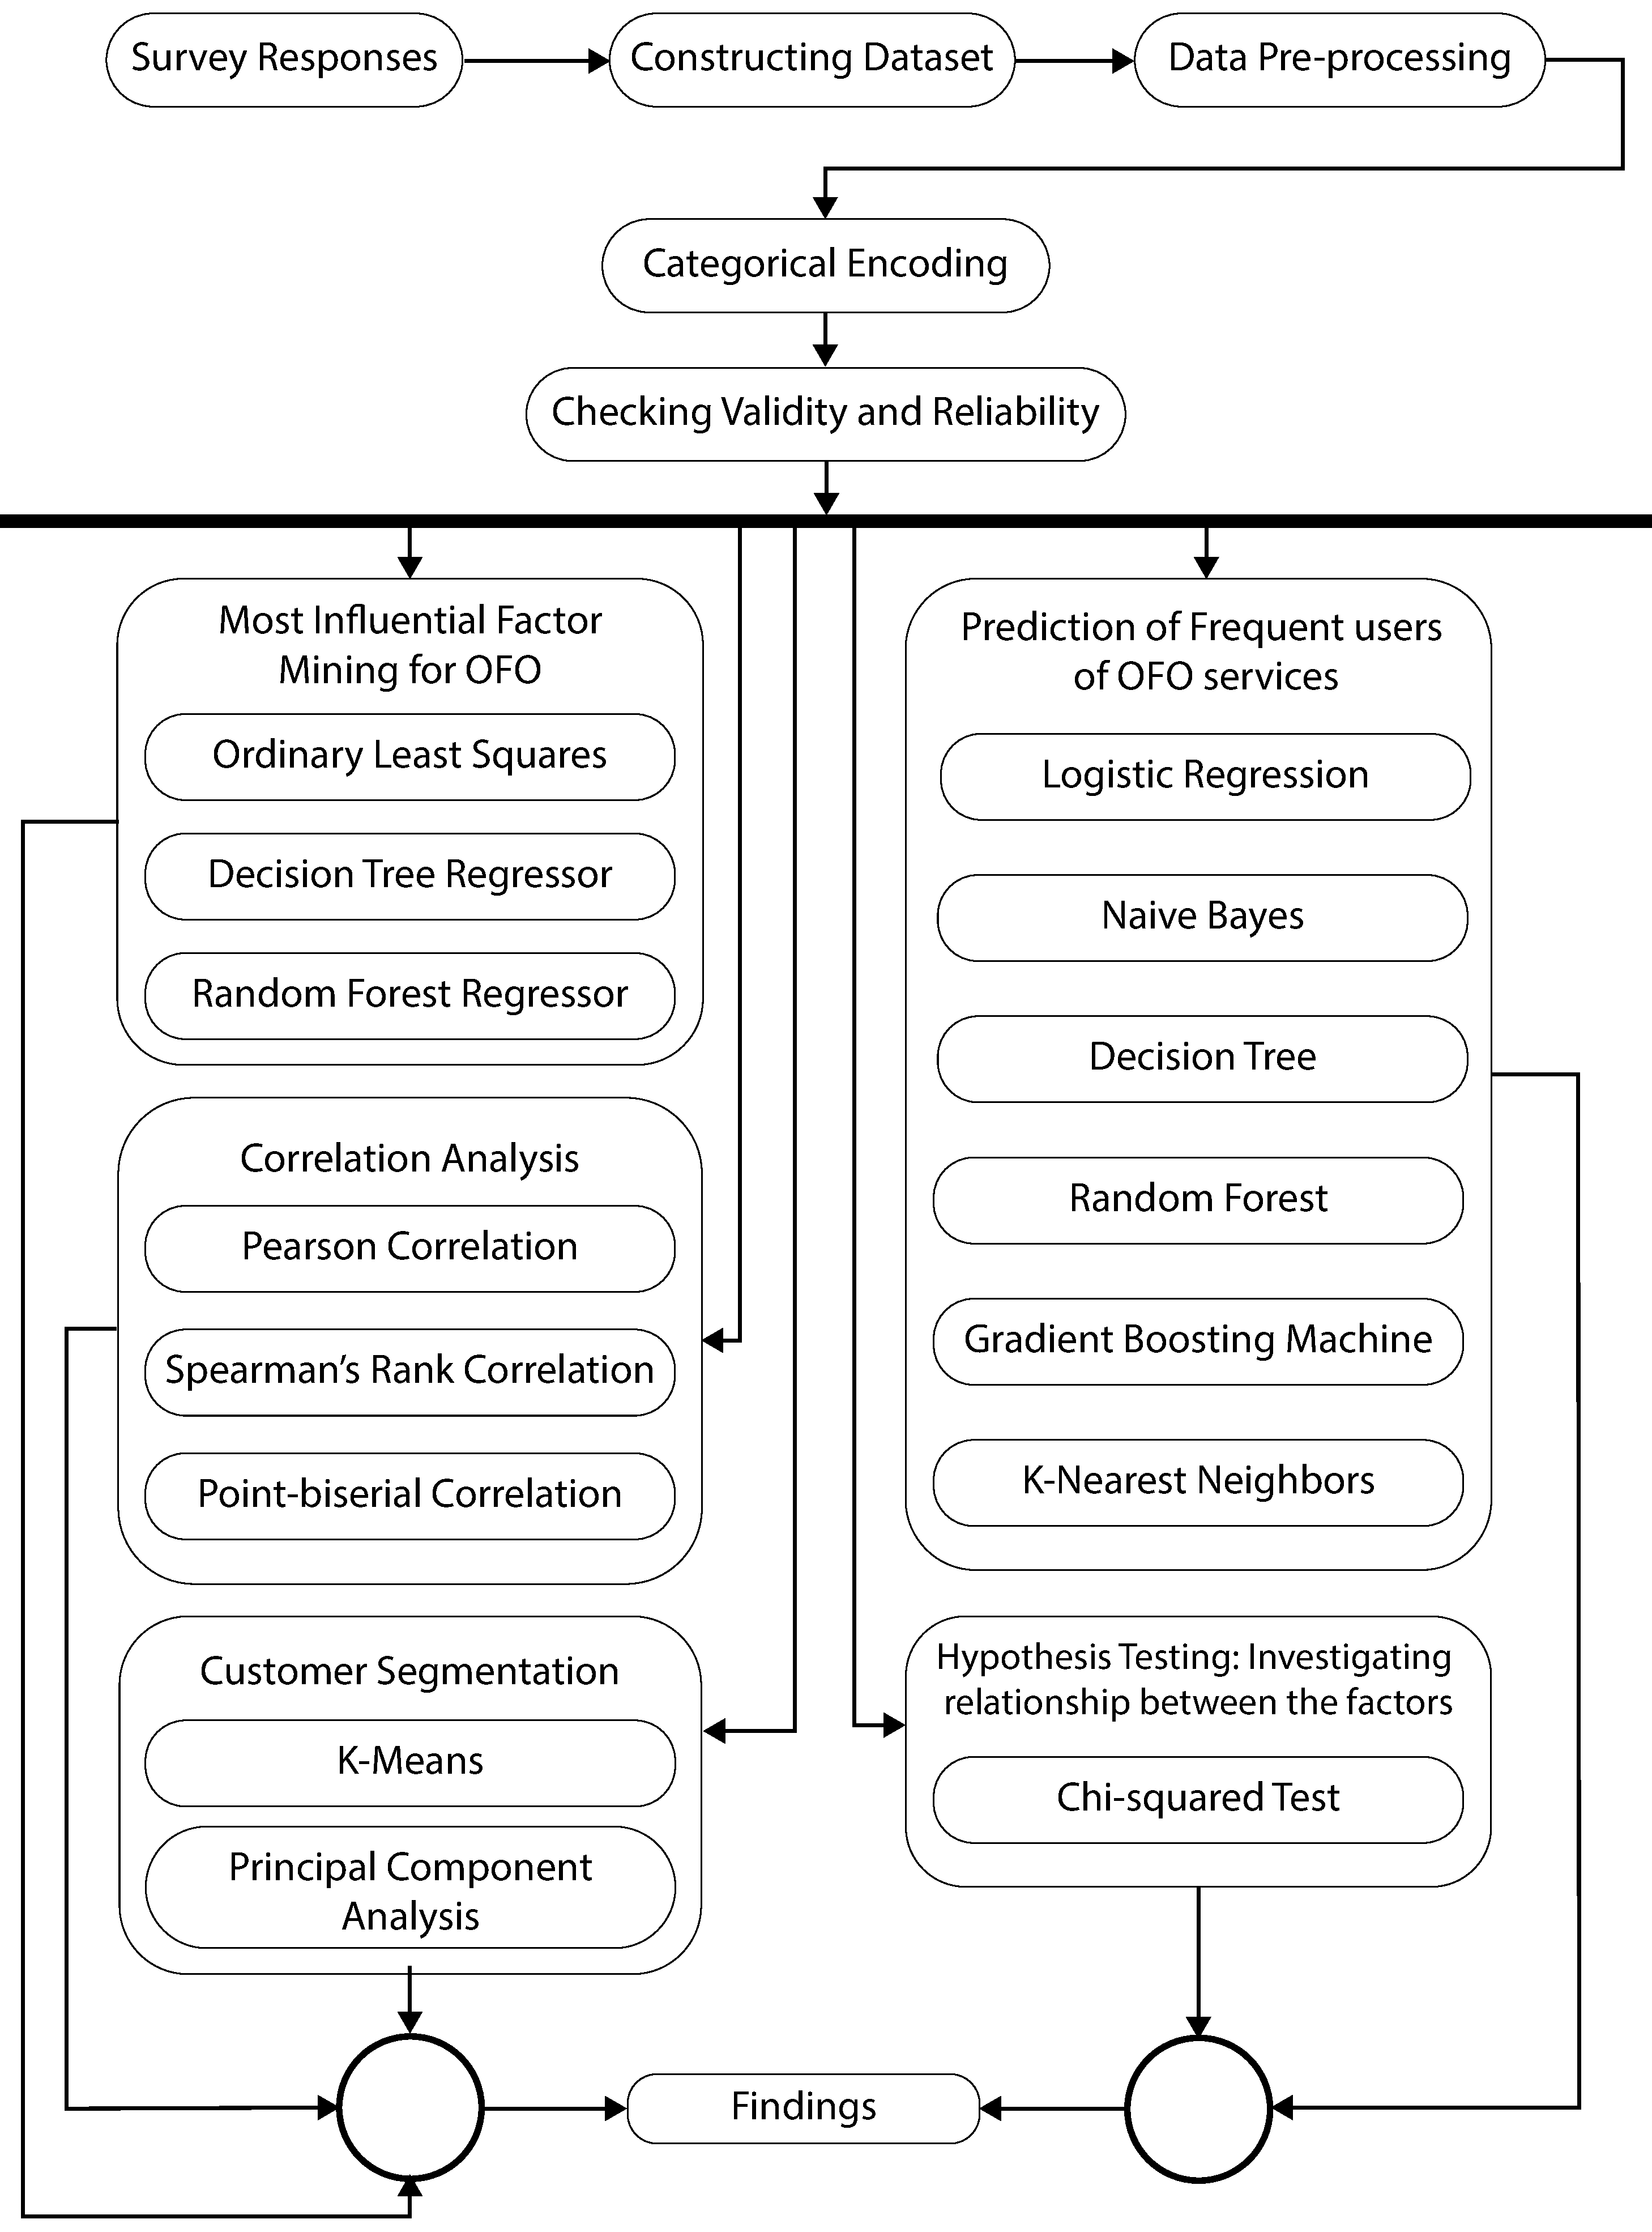
\includegraphics[scale = 0.25]{figs/workplan_v4.pdf}
  \caption{Top level overview of the proposed system.}
  \label{fig:workplan}
\end{figure}

In figure~\ref{fig:workplan}, we can see the top-level overview of our proposed system. We start by collecting responses from the survey and constructing our dataset. We do data pre-processing and test for validity and reliability. Then we do correlation analysis, find factors that influence the use of OFO services, create a prediction model, apply customer segmentation to our data and do some hypothesis testing. Finally, we show our findings.

\subsection{Data Collection}

To investigate the factors that influence the decision to order food online among individuals in Bangladesh, a survey is conducted. The survey questions are divided into two parts. One is the demographic data and the other is questions related to online food ordering and the factors influencing it. There were in total 25 questions in the questionnaire. The survey is done anonymously to protect the respondent's privacy. The survey is done through Google Forms and is designed to take the smallest amount of time possible. To accomplish that, we first share the form with our peers and take feedback from them. We incorporate the feedback and make it public. The questions ranged from text-based, multiple-choice questions (MCQ), checkboxes, and Likert scale questions.
% The survey questions are shared in the appendix. 

    \begin{table}[width=\linewidth,cols=2,pos=h]
    \caption{Questionnaire Description.}
    \begin{tabular*}{\tblwidth}{@{\extracolsep{\fill}}LL@{}}
    \hline
        Attributes & Data Type \\
        \hline
        Gender & Categorical Value \\
        Age & Numeric Ranges \\
        Weight & Numeric Value (Kilogram) \\
        Height & Numeric Value (Feet and Inches) \\
        Educational qualification & Categorical Value \\
        Employment status & Categorical Value \\
        Financial dependency & Categorical Value \\
        Marital status & Categorical Value \\
        Physical activity & Numeric Range: 1-7 (per week) \\
        Preferred OFO apps & Categorical Value \\
        OFO apps use duration & Categorical Value  \\
        Orders per month & Numeric Value \\
        Ordering time & Categorical Value \\
        Types of food ordered & Categorical Value \\
        Tries out new technologies & Likert Scale \\
        Makes impulsive decisions & Likert Scale\\
        Too busy to cook & Likert Scale\\
        Does not like to cook & Likert Scale\\
        Ordering online is easy & Likert Scale\\
        Variety of options & Likert Scale\\
        Ordering is inexpensive & Likert Scale\\
        Promo codes and discounts & Likert Scale \\
        Food is delivered quickly & Likert Scale \\
        Food is safe and hygienic & Likert Scale\\
        Food is nutritious & Likert Scale \\
        \hline
    \end{tabular*}
    \end{table}
    
Throughout the data collection period, we received several queries regarding why a respondent needs to log in to their email to respond to our questions. We explained to them that this is necessary to protect the survey from getting spam and random responses. Another concern we faced, was about the user being reluctant to share their personal information like height and weight we assured them that none of the answers were connected to their emails. We also made sure to not force anyone to share their information and only took responses if they gave it willingly. 

\subsection{Data pre-processing}
After collecting the survey responses, the column names are modified for improved readability and ease of use. The height variable, which was initially recorded in feet and inches, gets converted to meters for consistency. Using the converted height and weight variables, the BMI of each respondent is calculated. A new variable, BMI\_CAT, is created to store the categorical values of BMI, including "Underweight", "Normal", "Overweight" and "Obese". To maintain the focus on the target population of individuals aged 16-30, any responses from individuals outside of this age range are removed, as about 98\% of the data consists of individuals within this age group. The Likert scale data obtained from the questions related to various factors are encoded into ordinal numerical values for ease of analysis. This conversion allowed for a more accurate statistical analysis of the collected data. We remove any responses where orders per month are less than 1 since that information is not useful for our research problem. After pre-processing we ended up with valid 331 responses which we used to conduct the rest of our research. A sample set of the dataset after pre-processing can be seen in table~\ref{tab:dataset_sample}

% \begin{figure}[htb]
%   \centering
%   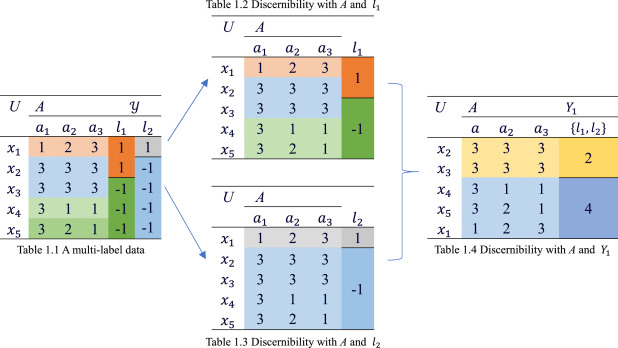
\includegraphics[width = \textwidth]{figs/features_attributes_values_relationship.jpg}
%   \label{fig:dataset_sample }
%   \caption{This figure is collected from \cite{che2020novel}, Pls use this type of diagram instead of the following,  for dataset availibility please deposit dataset in Mandeley or IEEE dataport etc}
% \end{figure}


% \begin{figure}[htb]
%   \centering
%   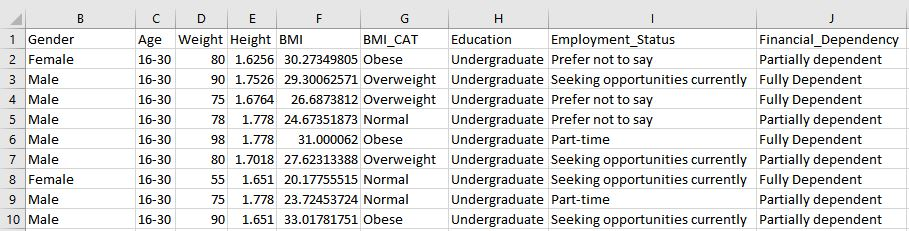
\includegraphics[width = \textwidth]{figs/dataset_screenshot_1.jpg}
%   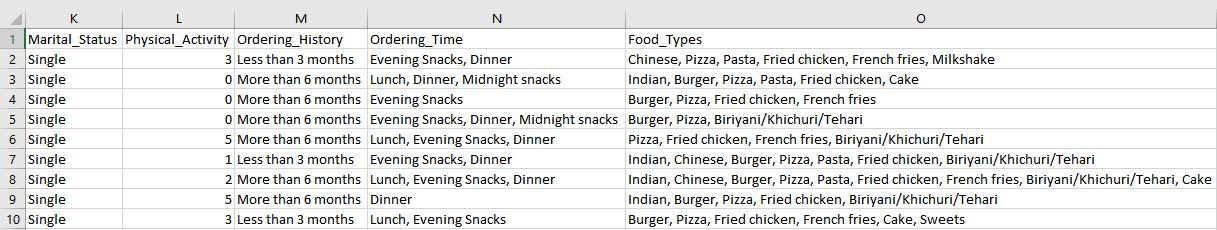
\includegraphics[width = \textwidth]{figs/dataset_screenshot_2.jpg}
%   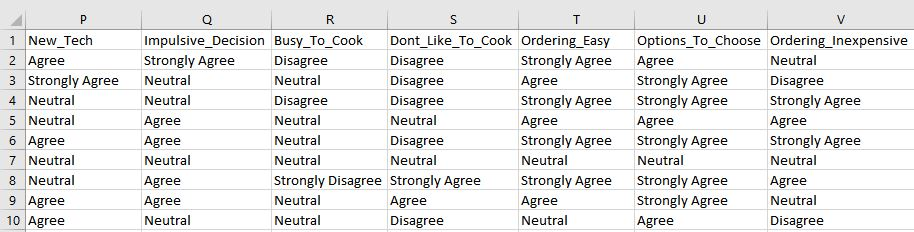
\includegraphics[width = \textwidth]{figs/dataset_screenshot_3.jpg}
%   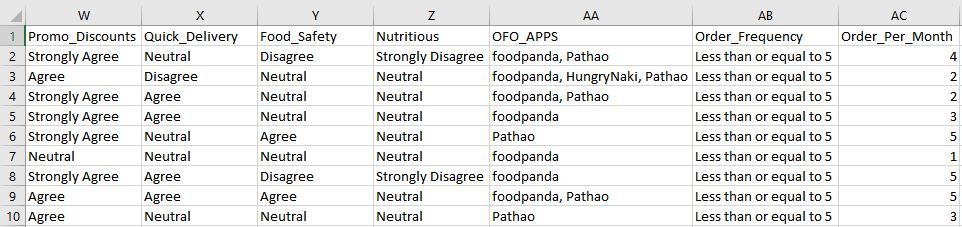
\includegraphics[width = \textwidth]{figs/dataset_screenshot_4.jpg}
%   \caption{Sample of the Dataset after pre-processing. Due to it's length the dataset is divided into four screenshots.}
%   \label{fig:dataset_sample}
% \end{figure}


% \begin{table}[htbp]
%   \centering
%   \caption{Demographic Information}
%   \label{tab:demographics}
%   \begin{tabular*}{\linewidth}{@{\extracolsep{\fill}}lccccllll@{}}
%     \toprule
%     Gender & Age & Weight & Height & BMI & BMI\_CAT & Education & Employment\_Status \\
%     \midrule
%     Female & 16-30 & 80 & 1.63 & 30.27 & Obese & Undergraduate & Prefer not to say \\
%     Male & 16-30 & 90 & 1.75 & 29.30 & Overweight & Undergraduate & Seeking opportunities \\
%     Male & 16-30 & 75 & 1.68 & 26.69 & Overweight & Undergraduate & Prefer not to say \\
%     Male & 16-30 & 78 & 1.78 & 24.67 & Normal & Undergraduate & Prefer not to say \\
%     Male & 16-30 & 98 & 1.78 & 31.00 & Obese & Undergraduate & Part-time \\
%     \bottomrule
%   \end{tabular*}
% \end{table}



% \begin{table}[htbp]
%     \centering
%     \caption{Ordering Information}
%     \label{tab:ordering_info}
%     \begin{tabular*}{\linewidth}{@{\extracolsep{\fill}}llcll@{}}
%         \toprule
%         Financial\_Dependency & Marital\_Status & Physical\_Activity & Ordering\_History & Ordering\_Time \\
%         \midrule
%         Partially dependent & Single & 3 & Less than 3 months & Evening Snacks, Dinner \\
%         Fully Dependent & Single & 0 & More than 6 months & Lunch, Dinner, Midnight snacks \\
%         Fully Dependent & Single & 0 & More than 6 months & Evening Snacks \\
%         Fully Dependent & Single & 5 & More than 6 months & Lunch, Evening Snacks, Dinner \\
%         Partially dependent & Single & 1 & Less than 3 months & Evening Snacks, Dinner \\
%         \bottomrule
%     \end{tabular*}
% \end{table}

% \begin{table}[htbp]
%     \centering
%     \caption{Food Preferences and Cooking Habits}
%     \label{tab:food_preferences}
%     \begin{tabular*}{\linewidth}{@{\extracolsep{\fill}}llllll@{}}
%         \toprule
%         Food\_Types & New\_Tech & Impulsive\_Decision & Busy\_To\_Cook\\
%         \midrule
%         Chinese, Pizza, Pasta, Fried chicken, French fries, Milkshake & Agree & Strongly Agree & Disagree\\
%         Indian, Burger, Pizza, Pasta, Fried chicken, Cake & Strongly Agree & Neutral & Neutral\\
%         Burger, Pizza, Fried chicken, French fries & Neutral & Neutral & Disagree\\
%         Burger, Pizza, Biriyani/Khichuri/Tehari & Neutral & Agree & Neutral\\
%         Pizza, Fried chicken, French fries, Biriyani/Khichuri/Tehari & Agree & Agree & Neutral\\
%         \bottomrule
%     \end{tabular*}
% \end{table}

% \begin{table}[htbp]
%     \centering
%     \caption{Ordering Preferences}
%     \label{tab:ordering_preferences}
%     \begin{tabular*}{\linewidth}{@{\extracolsep{\fill}}llllll@{}}
%         \toprule
%         Dont\_Like\_To\_Cook & Ordering\_Easy & Options\_To\_Choose & Ordering\_Inexpensive & Promo\_Discounts \\
%         \midrule
%         Disagree & Strongly Agree & Agree & Neutral & Strongly Agree \\
%         Disagree & Agree & Strongly Agree & Disagree & Agree \\
%         Disagree & Strongly Agree & Strongly Agree & Strongly Agree & Strongly Agree \\
%         Neutral & Agree & Agree & Agree & Strongly Agree \\
%         Disagree & Strongly Agree & Strongly Agree & Strongly Agree & Strongly Agree \\
%         \bottomrule
%     \end{tabular*}
% \end{table}

% \begin{table}[htbp]
%     \centering
%     \caption{Ordering Habits and Preferences}
%     \label{tab:ordering_habits}
%     \begin{tabular*}{\linewidth}{@{\extracolsep{\fill}}llllcc@{}}
%         \toprule
%         Quick\_Delivery & Food\_Safety & Nutritious & OFO\_APPS & Order\_Frequency & Order\_Per\_Month \\
%         \midrule
%         Neutral & Disagree & Strongly Disagree & foodpanda, Pathao & $\leq 5$ & 4 \\
%         Agree & Neutral & Neutral & foodpanda, Pathao & $\leq 5$ & 2 \\
%         Agree & Neutral & Neutral & foodpanda & $\leq 5$ & 3 \\
%         Neutral & Agree & Neutral & Pathao & $\leq 5$ & 5 \\
%         Neutral & Neutral & Neutral & foodpanda & $\leq 5$ & 1 \\
%         \bottomrule
%     \end{tabular*}
% \end{table}

\begin{table}[htbp]
    \centering
    \caption{Sample of the Dataset after pre-processing. Due to its length, the dataset is divided into 5 subtables.}
    \label{tab:dataset_sample}
    \begin{subtable}{\textwidth}
        \centering
        \begin{tabular*}{\linewidth}{@{\extracolsep{\fill}}lccccllll@{}}
            \toprule
            Gender & Age & Weight & Height & BMI & BMI\_CAT & Education & Employment\_Status \\
            \midrule
            Female & 16-30 & 80 & 1.63 & 30.27 & Obese & Undergraduate & Prefer not to say \\
            Male & 16-30 & 90 & 1.75 & 29.30 & Overweight & Undergraduate & Seeking opportunities \\
            Male & 16-30 & 75 & 1.68 & 26.69 & Overweight & Undergraduate & Prefer not to say \\
            Male & 16-30 & 78 & 1.78 & 24.67 & Normal & Undergraduate & Prefer not to say \\
            Male & 16-30 & 98 & 1.78 & 31.00 & Obese & Undergraduate & Part-time \\
            \bottomrule
        \end{tabular*}
        \caption{}
        \label{tab:sample_1}
    \end{subtable}

    \vspace{1em} % Adjust the vertical space between tables

    \begin{subtable}{\textwidth}
        \centering
        \begin{tabular*}{\linewidth}{@{\extracolsep{\fill}}llcll@{}}
            \toprule
            Financial\_Dependency & Marital\_Status & Physical\_Activity & Ordering\_History & Ordering\_Time \\
            \midrule
            Partially dependent & Single & 3 & Less than 3 months & Evening Snacks, Dinner \\
            Fully Dependent & Single & 0 & More than 6 months & Lunch, Dinner, Midnight snacks \\
            Fully Dependent & Single & 0 & More than 6 months & Evening Snacks \\
            Fully Dependent & Single & 5 & More than 6 months & Lunch, Evening Snacks, Dinner \\
            Partially dependent & Single & 1 & Less than 3 months & Evening Snacks, Dinner \\
            \bottomrule
        \end{tabular*}
        \caption{}
        \label{tab:sample_2}
    \end{subtable}

    \vspace{1em} % Adjust the vertical space between tables
    
    \begin{subtable}{\textwidth}
        \centering
        \begin{tabular*}{\linewidth}{@{\extracolsep{\fill}}llllll@{}}
            \toprule
            Food\_Types & New\_Tech & Impulsive\_Decision & Busy\_To\_Cook\\
            \midrule
            Chinese, Pizza, Pasta, Fried chicken, French fries, Milkshake & Agree & Strongly Agree & Disagree\\
            Indian, Burger, Pizza, Pasta, Fried Chicken, Cake & Strongly Agree & Neutral & Neutral\\
            Burger, Pizza, Fried chicken, French fries & Neutral & Neutral & Disagree\\
            Burger, Pizza, Biriyani/Khichuri/Tehari & Neutral & Agree & Neutral\\
            Pizza, Fried chicken, French fries, Biriyani/Khichuri/Tehari & Agree & Agree & Neutral\\
            \bottomrule
        \end{tabular*}
        \caption{}
        \label{tab:sample_3}
    \end{subtable}

    \vspace{1em} % Adjust the vertical space between tables
    
    \begin{subtable}{\textwidth}
        \centering
        \begin{tabular*}{\linewidth}{@{\extracolsep{\fill}}llllll@{}}
            \toprule
            Dont\_Like\_To\_Cook & Ordering\_Easy & Options\_To\_Choose & Ordering\_Inexpensive & Promo\_Discounts \\
            \midrule
            Disagree & Strongly Agree & Agree & Neutral & Strongly Agree \\
            Disagree & Agree & Strongly Agree & Disagree & Agree \\
            Disagree & Strongly Agree & Strongly Agree & Strongly Agree & Strongly Agree \\
            Neutral & Agree & Agree & Agree & Strongly Agree \\
            Disagree & Strongly Agree & Strongly Agree & Strongly Agree & Strongly Agree \\
            \bottomrule
        \end{tabular*}
        \caption{}
        \label{tab:sample_4}
    \end{subtable}

    \vspace{1em} % Adjust the vertical space between tables

    \begin{subtable}{\textwidth}
        \centering
        \begin{tabular*}{\linewidth}{@{\extracolsep{\fill}}llllcc@{}}
            \toprule
            Quick\_Delivery & Food\_Safety & Nutritious & OFO\_APPS & Order\_Frequency & Order\_Per\_Month \\
            \midrule
            Neutral & Disagree & Strongly Disagree & foodpanda, Pathao & $\leq 5$ & 4 \\
            Agree & Neutral & Neutral & foodpanda, Pathao & $\leq 5$ & 2 \\
            Agree & Neutral & Neutral & foodpanda & $\leq 5$ & 3 \\
            Neutral & Agree & Neutral & Pathao & $\leq 5$ & 5 \\
            Neutral & Neutral & Neutral & foodpanda & $\leq 5$ & 1 \\
            \bottomrule
        \end{tabular*}
        \caption{}
        \label{tab:sample_5}
    \end{subtable}
\end{table}

\subsection{Dataset Validity and Reliability}

Before applying all of the discussed methods we use Cronbach's Alpha~\cite{chronbach}, which is a way of assessing reliability by comparing the amount of shared variance, or covariance, among the items making up an instrument to the amount of overall variance. This is done to test the validity and reliability of our dataset. The idea is that if the instrument is reliable, there should be a great deal of covariance among the items relative to the variance. 

After applying Cronbach's Alpha on our dataset we get the value of 0.89. According to this paper by Taber~\cite{taber_2017} a Cronbach's alpha value higher than 0.70 is considered acceptable and above 0.80 and above is considered better. Therefore we can safely say that our dataset is valid and reliable. 

\subsection{Most Influential Factor Mining for OFO}

To find factors that are influencing a person to use OFO, we use Ordinary Least Squares (OLS)~\cite{ols}, Decision Tree Regressor~\cite{decision_tree} and Random Forest Regressor~\cite{random_forest}. 

% \subsubsection{Methods}

\paragraph{Ordinary Least Squares:}
This is a linear least squares method that chooses unknown parameters in a linear regression. This method tries to find the line that fits the data points the best by reducing the total amount of error between the predicted values and the actual values of the dependent variable. The model takes the form of an equation:

\begin{equation}
    y = b_0 + b_1x_1 + b_2x_2 + ... + b_nx_n
\end{equation}

where y is the dependent variable, $x_1$, $x_2$, ..., $x_n$ are the independent variables, and $b_0$, $b_1$, $b_2$, ..., $b_n$ are the coefficients of the equation. The goal of OLS is to find the values of the coefficients that minimize the difference between the predicted values of y (based on the equation) and the actual values of y. A system of linear equations is solved to find the coefficients. The matrix representation of this system is $X'Xb = X'y$, here X is the matrix of independent variables, b is the vector of coefficients and y is the vector of the dependent variable. These coefficients can tell us how strongly and in which way the independent variable affects the dependent variable. The one with the biggest coefficient is the most important factor in influencing the dependent variable. 

\paragraph{Decision Tree:} 
This method uses a tree-shaped model to make decisions and predict outcomes. The tree is created by splitting the data into smaller groups based on the values of the independent variables. This process is repeated recursively until we have subsets that can predict the consequences of each decision. At each internal node of the tree, a decision rule is applied to the data, and the tree branches accordingly. Once the tree is built, we use it to identify the most important variables for ordering food online by looking at the variables that are used in the decision rules at the top of the tree. 

\paragraph{Random Forest:}
This is an ensemble method that merges the predictions of multiple decision trees. To use this method, we first divide the data into different subsets. Then, we train multiple decision trees on each subset. Each tree makes its predictions based on the data it was trained on. Finally, we take the average of all the predictions from these trees to get the final result. Random forest is more robust to overfitting than a single decision tree, and it also allows us to identify the most important variables by looking at the variables that are used in the decision rules of the majority of the trees. 

The most important equation for Random Forest is the feature importance formula which is used to calculate the importance of each feature. The feature importance of a feature is calculated as the average decrease in impurity across all decision trees in the forest. The impurity can be calculated using the Gini Impurity.

\begin{equation}
    Gini = 1 - \sum_{i=1}^{m} p_i^2
\end{equation}

We use the 11 factors which are liking to try new technologies, making an impulsive decision, being too busy to cook, disliking cooking, finding ordering online to be easy, having a variety of options, finding ordering to be inexpensive, because of promotional offers and discounts, quick delivery, food safety and nutritious value. We use orders per month as the dependent variable. We calculate the mean and standard deviation of each factor. Then apply OLS, Decision Tree Regressor, and Random Forest Regressor. After that, we use the r-squared value to measure the goodness of fit of our regression models. The r-squared values for OLS, Decision Tree, and Random Forest are 0.64, 0.01 and 0.04. Which means OLS is a better approach for our data.

% \subsubsection{Results \& Findings}

% The results of the experiments which are done to find the most influencing factors are shown in table~\ref{tab:factors_results} gives us an idea on which factors influence a person to use OFO services. 

% \begin{table}[htb]
% \caption{Influential Factors in Online Food Orders: Comparing Mean, Standard Deviation, OLS, Decision Tree, and Random Forest Values.}
% \label{tab:factors_results}
% \begin{tabular*}{\linewidth}{@{\extracolsep{\fill}}lccccc@{}}
% \hline
%     Factors & Mean & SD & OLS & DT & RF \\
%     \hline
%     New Tech & 2.23 & 1.09 & 0.39 & 0.01 & 0.22 \\
%     Impulsive Decision & 2.01 & 1.16 & 0.90 & 0.34 & 0.22 \\
%     Busy To Cook & 2.12 & 1.16 & 0.18 & 0.05 & 0.10 \\
%     Don't Like To Cook & 1.82 & 1.25 & 0.33 & 0.01 & 0.13 \\
%     Ordering Easy & 2.98 & 0.95 & 0.65 & 0.11 & 0.08 \\
%     Options To Choose & 2.98 & 1.03 & 0.15 & 0.01 & 0.06 \\
%     Ordering Inexpensive & 1.62 & 1.10 & 0.27 & 0.22 & 0.07 \\
%     Promo Discounts & 2.60 & 1.12 & 0.33 & 0.01 & 0.09 \\
%     Quick Delivery & 2.28 & 1.00 & 0.11 & 0.01 & 0.05 \\
%     Food Safety & 1.79 & 0.86 & -0.40 & 0.01 & 0.05 \\
%     Nutritious & 1.45 & 0.98 & -0.32 & 0.28 & 0.09 \\
%     \hline
% \end{tabular*}
% \end{table}

% The mean values based on solely the responses from the respondents suggests that the most important factors in influencing people's decision to order food online are the convenience of ordering (mean score of 2.98), the variety of options available (mean score of 2.98), and promotional offers and discounts (mean score of 2.60). 

\subsection{Hypothesis Testing: Investigating the relationship between the factors}
In our study, we also conduct some hypothesis~\cite{stefanczyk2024cooks} testing using the chi-squared test~\cite{chi}. We use this test since the factors are categorical values and we want to see if the factors are independent of each other.

% \subsubsection{Method}

\paragraph{Chi-Squared Test:} This test is used to determine if there is a significant difference between an observed distribution and a theoretical distribution. The test statistic is calculated using the following equation:

\begin{align}
    \chi^2 = \sum_{i=1}^{n} \frac{(O_i - E_i)^2}{E_i}
\end{align}

Where:

O = observed frequency

E = expected frequency
\hfill \break

The degrees of freedom for the test is calculated as:

\begin{align}
df = (number \,of \,rows - 1) * (number \,of \,columns - 1)
\end{align}

The degrees of freedom (df) adjust for the information lost due to fixed marginal constraints within the contingency table. This adjustment ensures the proper chi-square distribution for calculating the p-value, henceforth controlling Type I error and preventing erroneous conclusions about the significance of observed associations between the variables.

The p-value is then looked up in a chi-squared distribution table with the corresponding degrees of freedom. If the calculated p-value is less than the chosen significance level (usually 0.05), then the null hypothesis (that there is no significant difference between the observed and theoretical distributions) is rejected, and it is concluded that there is a significant difference between the two. We use the chi-squared test of independence as the factors have ordinal values. So, something like Pearson’s correlation coefficient might not be the best measure of testing here as it assumes that the data is normally distributed and continuous. 

We test the following hypotheses for our study, 

People who are open to experimenting with new technology such as OFO services, may find it to be effortless to place an order. These platforms offer an easy-to-use and intuitive interface which simplifies the ordering process, thus allowing users to place orders quickly without any sort of hassle. Moreover, these applications often provide the option to track orders in real-time, personalized recommendations. All of these features can enhance the overall ordering experience and make it more convenient for the users to use. Based on this argument we come up with the following hypothesis: 

\textit{H1: There is a significant relationship between trying out new technology and thinking that using OFO service is easy.} 

People who have busy schedules may be more likely to make impulsive decisions when it comes to using OFO services. Due to their busy lifestyle, they may not have the energy to shop for ingredients or cook at home. Therefore, they may turn to quick and easy options such as ordering takeout. Based on this argument we come up with the following hypothesis: 

\textit{H2: There is a significant relationship between making impulsive decisions when using OFO service and being too busy to cook.} 

People who do not like to cook may appreciate the variety of options that are available on the OFO platforms. For them, the thought of preparing meals at home can be unappealing or they might prefer to have a variety of options to choose from when ordering food. Based on this argument we come up with the following hypothesis: 

\textit{H3: There is a significant relationship between people not liking to cook and finding there are many options to choose from when using OFO service.} 

Promotional offers or discounts can make the use of OFO services more cost-effective for users. These offers can take various forms such as coupons, loyalty programs, and special deals. These can be used to reduce the cost of items, delivery fees or sometimes even the entire order. By making use of these discounts, customers can save money on their orders. Therefore, this leads them to believe that ordering food online is inexpensive. Based on this argument we come up with the following hypothesis: 

\textit{H4: There is a significant relationship between thinking OFO service is inexpensive and ordering food because of promo codes and discounts.} 

\begin{table}[htb]
\caption{Results of Hypothesis Testing.}
\begin{tabular*}{\linewidth}{@{\extracolsep{\fill}}lcl@{}}
\toprule
Serial & P-Value & Decision \\
\midrule
% H1 & New Tech - Ordering Easy & $<$ 0.001 & Accepted \\
% H2 & Busy To Cook - Impulsive Decision & 0.114 & Rejected \\
% H3 & Options To Choose - Don't Like To Cook & $<$ 0.001 & Accepted \\
% H4 & Ordering Inexpensive - Promo Discounts & $<$ 0.001 & Accepted \\
H1 & $<$ 0.001 & Accepted \\
H2 & 0.114 & Rejected \\
H3 & $<$ 0.001 & Accepted \\
H4 & $<$ 0.001 & Accepted \\
\bottomrule
\end{tabular*}
\end{table}

% \subsubsection{Results \& Findings:}

% The results of the hypothesis study point out that the first hypothesis, H1 is accepted and the null hypothesis is rejected as the p-value is $<$ 0.001, which is less than ($\alpha$ = 0.05). This means that people who tend to try out new technologies also feel that ordering food online is really convenient and easy. 

% For the second hypothesis, H2 is rejected as the p-value (0.1143) is higher than the $\alpha$ (0.05). This means we could not find any significant relationship between being too busy to cook and making impulsive decisions when ordering food online. 

% The third hypothesis, H3 is accepted and the null hypothesis is rejected as the p-value ($<$ 0.001) is lower than the $\alpha$ (0.05). This means there is a significant relationship between having many options to choose from when ordering food online and not liking to cook. 

% And the fourth hypothesis, H4 is accepted and the null hypothesis is rejected as the p-value ($<$ 0.001) is less than the $\alpha$ (0.05). This means that there exists a significant relationship between finding ordering food online to be inexpensive and using promo codes and discounts when ordering food online. 

\subsection{Correlation Analysis}

To examine the relationship between BMI (x) and the frequency of ordering food online (y), we apply several correlation analysis methods. These are Pearson Correlation~\cite{pearson} where we use the actual BMI value of a respondent, Spearman's Rank Correlation~\cite{spearman} where the BMI categories are used and Point-biserial Correlation~\cite{point_biserial} where we convert BMI categories to binary categories. 

% \subsubsection{Methods}

\paragraph{Pearson correlation:}
This method measures the linear relationship between two continuous variables. The process involves calculating the means ($\bar{x}, \Bar{y}$) and standard deviations of each variable, followed by computing the product of the deviations of each variable from its mean for each data point. The following equation is then used to calculate Pearson's correlation coefficient, r: 

\begin{equation}
    r = \frac{\sum\limits_{i=1}^{n} (x_i - \bar{x})(y_i - \bar{y})}{\sqrt{\sum\limits_{i=1}^{n} (x_i - \bar{x})^2}\sqrt{\sum\limits_{i=1}^{n} (y_i - \bar{y})^2}}
\end{equation}

The resulting value of r ranges from -1 to 1, here -1 indicates a perfect negative linear relationship, 0 indicates no linear relationship, and 1 indicates a perfect positive linear relationship. To evaluate the significance of the correlation coefficient, a p-value is determined using the correlation coefficient, degrees of freedom (df = n-2), and a significance level of $\alpha$ = 0.05 is used usually. The table of critical values is used to find the p-value. The correlation coefficient is assumed as zero by the null hypothesis, implying that there is no correlation between the two variables. The alternative hypothesis is that the correlation coefficient is not zero, implying that there is a correlation between the two variables. If the p-value is less than $\alpha$, we get enough evidence to accept the alternative hypothesis and reject the null hypothesis. This method is applicable when both variables are continuous and assumes the data follow a normal distribution. It also assumes the observations are independent of each other. 

\paragraph{Spearman's rank correlation coefficient:}
This is a non-parametric way of measuring correlation. With this, we can measure how well the relationship between two variables can be described by using a monotonic function. It is similar to Pearson correlation but instead of measuring linear association, this evaluates rank order similarity between variables. 

In this method, each variable is assigned ranks based on its values. The smallest value receives a rank of 1, the second smallest a rank of 2 and so on. Then it determines the difference between ranks for each paired observation and these differences represent the change in the variables' relative positions. Each difference obtained in the previous step is then squared to stop the positive and negative differences cancelling each other out. Finally, the coefficient is calculated using the following formula:

\begin{equation}
    \rho = 1 - \frac{(6 * sum\ of\ squared\ differences)}{n * n^{2-1}}
\end{equation}

The results will range from -1 to 1, where a  value of +1 indicates that as one variable increases, the other variable also increases consistently. On the other hand, a value of -1 means that as one variable increases, the other variable decreases consistently. A coefficient of 0 suggests no monotonic relationship between the variables. This approach only works when the variables are ordinal or ranked. This method is also less sensitive to outlier data. 

\paragraph{Point-biserial correlation:}
This approach measures the strength and direction of association between a continuous variable and a binary variable. 

At first, the data is divided into two groups based on the binary variable. One group represents the presence of the characteristic while the other group represents the absence of it. Then, the mean value of the continuous variable is calculated for each group separately. After that, the standard deviation of the whole dataset is calculated, disregarding the grouping which represents the variability of the continuous variables across the entire dataset. The mean of the group representing the absence of the characteristic is then subtracted from the mean of the group representing the presence of it. We divide the difference by the standard deviation. We then get the point-biserial correlation coefficient which quantifies the strength and direction of the relationship between the continuous and binary variable.

The coefficient value ranges from -1 to +1. A positive value indicates a positive relationship, meaning higher values of the continuous variable tend to be associated with the presence of the characteristic. A negative value indicates a negative relationship, where higher values of the continuous variable tend to be associated with the absence of the characteristic. A value of 0 indicates no relationship between the continuous variable and the binary variable. This approach assumes that the continuous variable follows a normal distribution or at least approximate normality. Skewed or variable with outliers may affect the accuracy. The observations should also be independent of each other. Larger sample sizes tend to yield more accurate estimates. 

For Pearson correlation, we use the BMI with continuous values and orders per month which also consists of continuous values. When using Spearman's rank correlation coefficient we use the categorical values of BMI instead and for Point-biserial correlation, we divide the BMI categories into binary groups such as not obese and obese, not normal weight and normal weight and apply the method. 

We also apply Pearson and Spearman's correlation on physical activity and orders per month. Treating the values for physical activity as continuous for Pearson and categorical for Spearman's.

\begin{table}[htb]
    \caption{Pearson and Spearman Correlation Test Results of BMI vs Orders Per Month.}
    \label{tab:pearson_spearman_bmi_OPM}
    \begin{tabular*}{\linewidth}{@{\extracolsep{\fill}}lccl@{}}
        \toprule
        Test & P-value & Coefficient & Relationship \\
        \midrule
        Pearson & $2.43^{-7}$ & 0.28 & Weak Positive \\
        Spearman & 0.003 & 0.15 & Very Weak Positive \\
        \bottomrule
    \end{tabular*}
\end{table}

% \subsubsection{Results \& Findings}

% The results from Pearson correlation and Spearman's rank correlation which was done between BMI and orders per month, gives us p-value of $2.43^{-7}$ and $0.003$ respectively, which suggests that there exists a statistically significant positive correlation between the two variables since both these values are less than 0.05. The coefficients values are $0.28$ and $0.15$ respectively which suggests there exists a weak positive correlation and a very weak positive correlation~\cite{jaadi_2019}. 


% \begin{table}[htb]
%     \caption{Results of Point-biserial Correlation on BMI vs Orders Per Month.}
%     \label{tab:Pbi_BMI_OPM}
%     \begin{tabular*}{\linewidth}{@{\extracolsep{\fill}}lccr@{}}
%         \toprule
%         BMI & P-value & Coefficient & Relationship \\
%         \midrule
%         Underweight & 0.84 & -0.01 & Rejected \\
%         Normal & $1.97^{-5}$ & -0.23 &  Weak Negative \\
%         Overweight & 0.04 & 0.04 & Very Weak Positive \\
%         Obese & $1.13^{-10}$ & 0.34 & Weak Positive \\
%         \bottomrule
%     \end{tabular*}
% \end{table}


% The results of shown on table~\ref{tab:Pbi_BMI_OPM} suggests that due to insufficient p-value any relation between Underweight and orders per month is rejected, normal weight has a weak negative relationship, overweight has a very weak positive relationship and obese has a weak positive relationship. 


% \begin{table}[htb]
%     \caption{Results of Correlation analysis between physical activity and orders per month.}
%     \label{tab:pearson_spearman_phy_OPM}
%     \begin{tabular*}{\linewidth}{@{\extracolsep{\fill}}lccr@{}}
%         \toprule
%         Test & P-value & Coefficient & Relationship \\
%         \midrule
%         Pearson & 0.026 & -0.12 & Very Weak Negative \\
%         Spearman & 0.085 & -0.10 & Rejected \\
%         \bottomrule
%     \end{tabular*}
% \end{table}


% As seen on table~\ref{tab:pearson_spearman_phy_OPM}, we can see that there exists a very weak negative relation between physical activity and orders per month which suggests that people who tend to order more may exercise less. However, the results from spearman's test is rejected as the p-value is 0.085, which is greater than the $\alpha$ value of 0.05.


% \begin{table}[htb]
%     \caption{Results of Point-biserial Correlation on Ordering History and Orders Per Month.}
%     \label{tab:Pbi_OH_OPM}
%     \begin{tabular*}{\linewidth}{@{\extracolsep{\fill}}lccl@{}}
%         \toprule
%         Ordering History & P-value & Coefficient & Relationship \\
%         \midrule
%         < 3 months & $1.40^{-5}$ & -0.23 & Weak Negative \\
%         3 - 6 months & 0.66 & 0.02 &  Rejected \\
%         > 6 months & $<$0.0001 & 0.18 & Very Weak Positive \\
%         \bottomrule
%     \end{tabular*}
% \end{table}


% The results of correlation analysis between ordering history and orders per month as seen on table~\ref{tab:Pbi_OH_OPM} shows that people who have been using OFO for more than 6 months tend to order more. The coefficient value of -0.23 suggests that there exists a weak relationship between ordering frequency and people who have been using this type of service for less than 3 months. However, due to the p-value (0.66) being higher than the $\alpha$ value of 0.05, any relationship between people who have been ordering for 3-6 months is rejected. 

\subsection{Prediction of Frequent users of OFO services}

To classify frequent users of OFO services we use several methods such as Logistic Regression~\cite{cox1958regression}, Naive Bayes~\cite{naive_bayes}, Decision Tree Classifier~\cite{decision_tree}, Random Forest Classifier~\cite{random_forest}, Gradient Boosting Machines (GBM)~\cite{gbm} and K-Nearest Neighbour (KNN)~\cite{knn}. 

% \subsubsection{Methods}

\paragraph{Logistic Regression:}
This is a commonly used statistical model for tasks that involve classifying things into two categories. The main aim is to predict the probability of an instance belonging to a specific class. Unlike linear regression, which predicts continuous values, it is specifically designed to predict the probability of an event happening. Instead of providing a direct numerical output, this method calculates the likelihood of an event occurring based on the input variables. This makes it suitable for tasks where we are interested in determining the likelihood or probability of a specific outcome. 

Logistic Regression models the relationship between the predictor variables and the output class probabilities using a logistic function or sigmoid function. The sigmoid function is defined as:

\begin{equation}
    S(z) = \frac{1}{1 + e^{-z}}
\end{equation}
Here, z represents a linear combination of the input features and model parameters. 

The model is trained by finding the optimal values for the model parameters which minimize the error between the predicted probabilities and the actual class labels in the training data. This is typically done using optimization algorithms such as Newton's method or Gradient Descent. The objective is to minimize the log loss of the predicted probabilities or maximize the likelihood of it. Once the model is trained and the optimal parameters are obtained, we can use the model to make predictions on new, unseen data. The sigmoid function is applied to the linear combination of the input features and parameters to obtain the predicted probability. A common threshold (0.5) is then used to classify the instance into one of the two classes based on the predicted probability. If the predicted probability is above the threshold, it is classified as class 1; otherwise, it is classified as class 0. 

\paragraph{Naive Bayes:}
This algorithm is built upon Bayes' theorem and assumes that given the class label, the features are conditionally independent of each other. 

This algorithm starts by calculating the prior probabilities of each class in the dataset. The prior probability of a class is the probability of encountering that class in the dataset without considering any feature information. For each feature in the dataset, this method calculates the conditional probability of observing that feature given a specific class label. This is done by counting the occurrences of each feature in the training samples belonging to a particular class. Once the prior probabilities and conditional probabilities are computed, Bayes' theorem is applied to calculate the posterior probability of each class given the observed features. Finally, the classifier predicts the class label for a new, unseen sample by selecting the class with the highest posterior probability.

The algorithm for Decision Tree and Random Forest classifier works in the same as the regressor approach but the classifier is more suitable for categorical or discrete class labels. 

\paragraph{Gradient Boosting Machines:}
This algorithm combines multiple weak predictive models (usually decision trees) to create a better predictive model. It is an ensemble learning method that sequentially builds an additive model by minimizing a predefined loss function using gradient descent. 

A weak learner which usually is a decision tree with a small depth which is also called a decision stump, is fitted to the training data. The tree is trained to minimize the loss function with respect to the target variable. The predictions of the weak learner are then subtracted from the true values of the target variable to obtain the residuals. The residuals represent the errors or the parts of the target variable that the model has not yet captured. Another weak learner is then fitted to the residuals obtained from the previous step. The goal is to find a new model that can capture the remaining patterns in the data that the previous model missed. The new weak learner is now added to the ensemble by combining it with the previous models. To combine the models, a weight is assigned to each weak learner, this is also known as the learning rate. The weight determines the contribution of each model to the final prediction. The process of calculating residuals, fitting the next learner and updating of the model is repeated iteratively for a specified number of times or until a predefined stopping criterion is met. In each iteration, a new weak learner is fitted to the negative gradients of the ensemble model built so far. The final prediction is gained by summing the predictions of all the weak learners with their respective weights. The model assigns higher weights to the more accurate learners, which allows it to give more importance to their predictions.

\paragraph{K-Nearest Neighbour:}
KNN is an algorithm that does not rely on any assumptions about the underlying data distribution. The fundamental idea behind KNN is to classify or predict the target variable of a new data point based on the majority vote or the average of the target variables of its K number of nearest neighbours in the feature space. 

At first, the value of K is figured out, which represents the number of nearest neighbours to consider for classification or regression. The optimal value of K can be found using techniques such as cross-validation or grid search. To classify or predict a new data point, the distance between that point and every other data point in the training data is calculated. The distance can be calculated using different metrics such as Manhattan distance and Euclidean distance. The distances are then sorted in ascending order and the K data points are selected with the shortest distances as the nearest neighbors. Then, the class label is determined that occurs most frequently among the K nearest neighbours. This can be done by counting the occurrences of each class label and selecting the one with the highest count. Once the class label or predicted value has been determined, it is assigned as the output for the new data point.

We divide the orders per month variable into two categories. One with less or equal to 5 orders per month which covers 56\% of the sample and another with more than 5 orders per month which covers the rest of 44\% of the sample. We then use this as the target label against all the features available in our dataset. We use univariate methods such as the Chi-squared test and ANOVA F-value to do some feature selection.
% We scale the data, select the best features using a correlation heat map, and implement the algorithms.

\begin{table}[htb]
\caption{Results of feature selection.}
\label{tab:feature_selection}
\begin{tabular*}{\linewidth}{@{\extracolsep{\fill}}ll@{}}
\toprule
Chi-squared Test     & ANOVA F-value            \\ 
\midrule
Gender               & Gender                   \\
BMI                  & BMI                      \\
Employment Status    & Employment Status        \\
Financial Dependency & Financial Dependency     \\
Physical Activity    & Marital Status           \\
Ordering History     & Physical Activity        \\
Impulsive Decision   & Ordering History         \\
Busy To Cook         & Impulsive Decision       \\
Dont Like To Cook    & Busy To Cook             \\
Ordering Easy        & Dont Like To Cook        \\
Options To Choose    & Ordering Easy            \\
Ordering Inexpensive & Options To Choose        \\
Promo Discounts      & Promo Discounts          \\
Quick Delivery       & Quick Delivery           \\
Food Safety          & Food Safety              \\
Nutritious           & Nutritious               \\ 
\bottomrule
\end{tabular*}
\end{table}

From table~\ref{tab:feature_selection}, we can see that 15 out of the 16 selected features are common for both methods. Therefore, we use these 15 to build our prediction models. 

We use several evaluation metrics like accuracy score, precision, recall, and F1-score to find the model with the best results.

% \subsubsection{Results \& Findings:}

% The results of the prediction model can be seen on table~\ref{tab:pred_before}.

% \begin{table}[htb]
%     \caption{Comparison of results among prediction models before feature selection.}
%     % \caption{Comparison of results among prediction models}
%     \label{tab:pred_before}
%     \begin{tabular*}{\linewidth}{@{\extracolsep{\fill}}lcccc@{}}
%         \toprule
%         Model & Accuracy & Precision & Recall & F1-Score \\
%         \midrule
%         LR  & 0.78 & 0.66 & 0.59 & 0.61 \\
%         NB  & 0.64 & 0.53 & 0.53 & 0.53 \\
%         DT  & 0.63 & 0.45 & 0.45 & 0.45 \\
%         RF  & 0.81 & 0.78 & 0.59 & 0.60 \\
%         GBM & 0.78 & 0.66 & 0.59 & 0.61 \\
%         KNN & 0.78 & 0.67 & 0.64 & 0.65 \\
%         \bottomrule
%     \end{tabular*}
% \end{table}


% We can see that out of 6 models, Random Forest performs the best with 81\% accuracy. whereas Naive Bayes performed worst with 64\% accuracy. Random Forest also has the best precision score of 0.78 which means it has a high level of precision in identifying positive instances. On the other hand, KNN correctly identified 64\% of the positive instances as seen on the Recall column.

% \begin{table}[htb]
%     \caption{Comparison of results among prediction models after feature selection.}
%     \label{tab:pred_after}
%     \begin{tabular*}{\linewidth}{@{\extracolsep{\fill}}lcccc@{}}
%         \toprule
%         Model & Accuracy & Precision & Recall & F1-Score \\
%         \midrule
%         LR  & 0.81 & 0.74 & 0.61 & 0.63 \\
%         NB  & 0.67 & 0.55 & 0.55 & 0.55 \\
%         DT  & 0.61 & 0.49 & 0.49 & 0.49 \\
%         RF  & 0.81 & 0.78 & 0.59 & 0.60 \\
%         GBM & 0.78 & 0.65 & 0.57 & 0.58 \\
%         KNN & 0.81 & 0.73 & 0.64 & 0.66 \\
%         \bottomrule
%     \end{tabular*}
% \end{table}

\subsection{Customer Segmentation}

Customer segmentation is a technique in data analysis to group customers based on their similarities and differences. One way of doing this is using the K-Means clustering algorithm~\cite{kmeans}, which is an unsupervised machine learning algorithm that aims to divide a given dataset into K distinct clusters, where each data point goes to the cluster with the nearest mean value. Principal Component Analysis (PCA)~\cite{Jolliffe2011} is a technique that can be used to reduce the dimension of the dataset.

% \subsubsection{Methods}

\paragraph{K-Means:}
The algorithm works by assigning data points iteratively to the cluster with the closest centroid and then updating the centroids to be the average of the data points in each cluster. This process continues until the centroids no longer change significantly.

The number of clusters K is usually chosen by using the Elbow method or silhouette scores. Then the the centroids of the clusters are initialized. This is done randomly or by using some other method, such as k-means++. Each data point then gets assigned to the cluster with the closest centroid. The centroids get updated to be the average of the data points in each cluster. This is repeated until the centroids no longer change significantly. 

\paragraph{Principal Component Analysis:}
This is a widely used statistical technique for dimensionality reduction and data analysis. It aims to find the directions or principal components in which the data varies the most and represents the data in a lower-dimensional space while preserving the essential information.

At first, the dataset is standardized to have a unit variance and zero mean. This step ensures that all features are on a similar scale and prevents variables with large variances from dominating the analysis. Then the covariance matrix of the standardized data is computed. The covariance matrix indicates the relationships between different features and measures how they vary together. The value in the $i^{th}$ row and $j^{th}$ column of the covariance matrix represents the covariance between the $i^{th}$ and $j^{th}$ features. An eigendecomposition is performed on the covariance matrix to find its eigenvalues and corresponding eigenvectors. The amount of variance explained by each principal component is represented by the eigenvalues. The eigenvectors represent the directions of these components. The eigenvalues indicate the relative importance of each principal component. PCA typically sorts the eigenvalues in descending order and selects the top-k eigenvectors corresponding to the largest eigenvalues, where k is the desired number of dimensions in the reduced space. The selected eigenvectors form a new coordinate system. The original data is projected onto this new coordinate system to obtain the reduced-dimensional representation. This projection involves multiplying the standardized data matrix by the eigenvector matrix, resulting in a transformed dataset with reduced dimensions. 

For this, we use only the 11 factors we developed that influence OFO to do customer segmentation. We use the K-Means~\cite{kmeans} algorithm to create the segmentation. We apply K-Means using both Principal Component Analysis (PCA)~\cite{Jolliffe2011} and one without using it. Before applying PCA, we use Kaiser-Meyer-Olkin test (KMO)~\cite{Kaiser1970} and Bartlett's Test of Sphericity~\cite{bartlett1950tests} to check if the data is suitable to apply PCA. The KMO test measures the proportion of variance in each variable that is explained by other variables, while Bartlett's Test confirms whether the correlations between variables are significantly different from zero. These tests help us avoid applying PCA to data where variables are entirely unrelated or where common factors are minimal, leading to unreliable results. The results of the KMO test give us 0.85 which makes it sufficient to perform factor analysis according to this paper~\cite{kmo}. The result of Bartlett's Test of Sphericity gives us a p-value of $1.06^{-228}$ which is lower than the $\alpha$ value of 0.05 and a high chi-squared value of 1301.43. Therefore, we can apply PCA to our data.

% We use elbow method and silhouette score to find optimal number of clusters. From figures~\ref{fig:elbow}, \ref{fig:elbow_pca}, \ref{fig:silhouette} and \ref{fig:silhouette_pca} we can see that the optimal number of clusters is 2.

% \begin{figure}[htb]
%   \centering
%   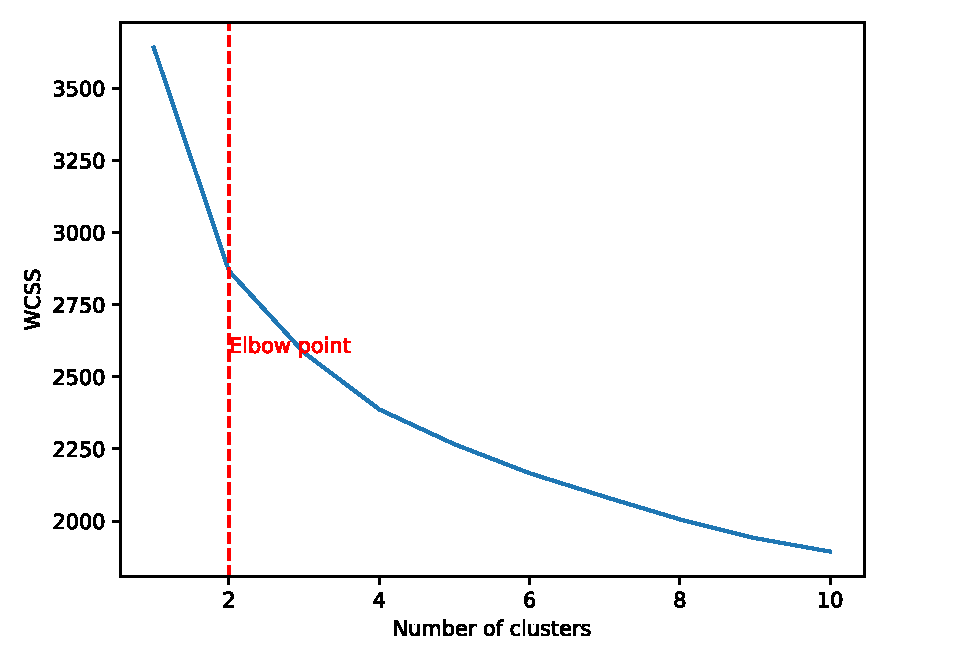
\includegraphics[width = \textwidth]{figs/elbow_plot.pdf}
%   \caption{Elbow method for determining the optimal number of clusters.}
%   \label{fig:elbow}
% \end{figure}

% \begin{figure}[htb]
%   \centering
%   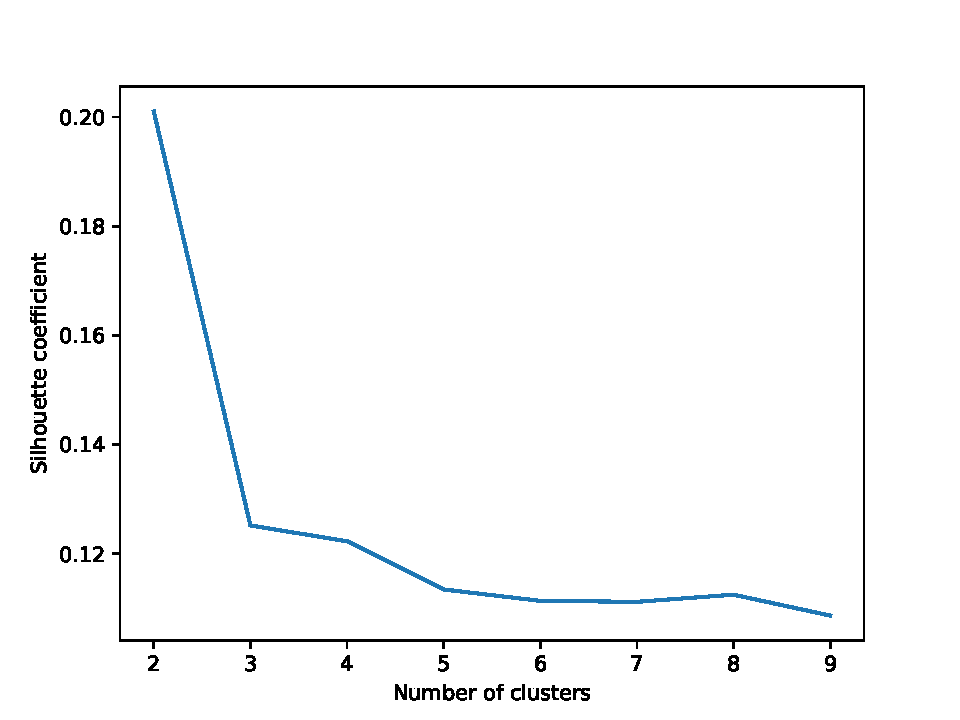
\includegraphics[width = \textwidth]{figs/silhouette_plot.pdf}
%   \caption{Silhouette plot for determining the optimal number of clusters.}
%   \label{fig:silhouette}
% \end{figure}

% \begin{figure}[htb]
%   \centering
%   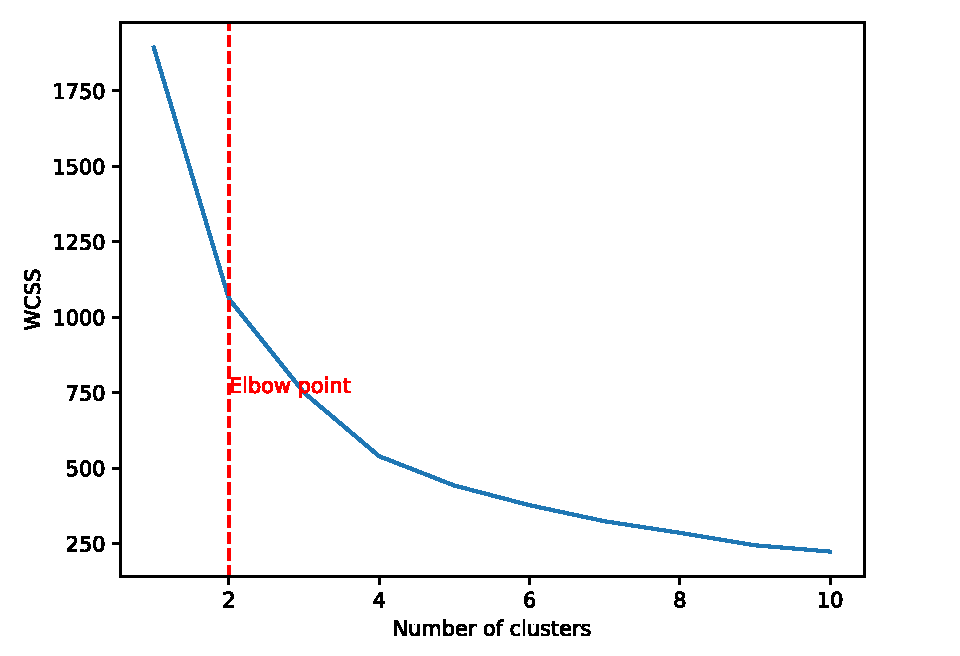
\includegraphics[width = \textwidth]{figs/elbow_plot_PCA.pdf}
%   \caption{Elbow method for determining the optimal number of clusters with PCA.}
%   \label{fig:elbow_pca}
% \end{figure}

% \begin{figure}[htb]
%   \centering
%   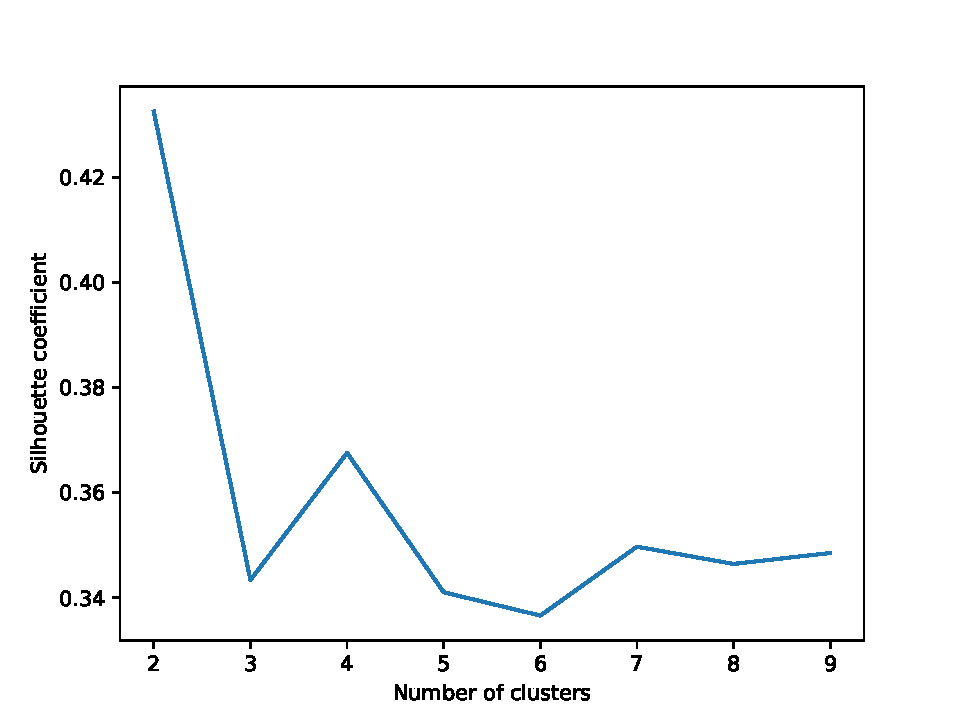
\includegraphics[width = \textwidth]{figs/silhouette_plot_PCA.pdf}
%   \caption{Silhouette plot for determining the optimal number of clusters with PCA.}
%   \label{fig:silhouette_pca}
% \end{figure}

We use the Elbow method and silhouette score to find an optimal number of clusters. From figures~\ref{fig:elbow+silhouette} and \ref{fig:elbow+silhouette_PCA} we can see that the optimal number of clusters is 2.

\begin{figure}[htb]
  \centering
  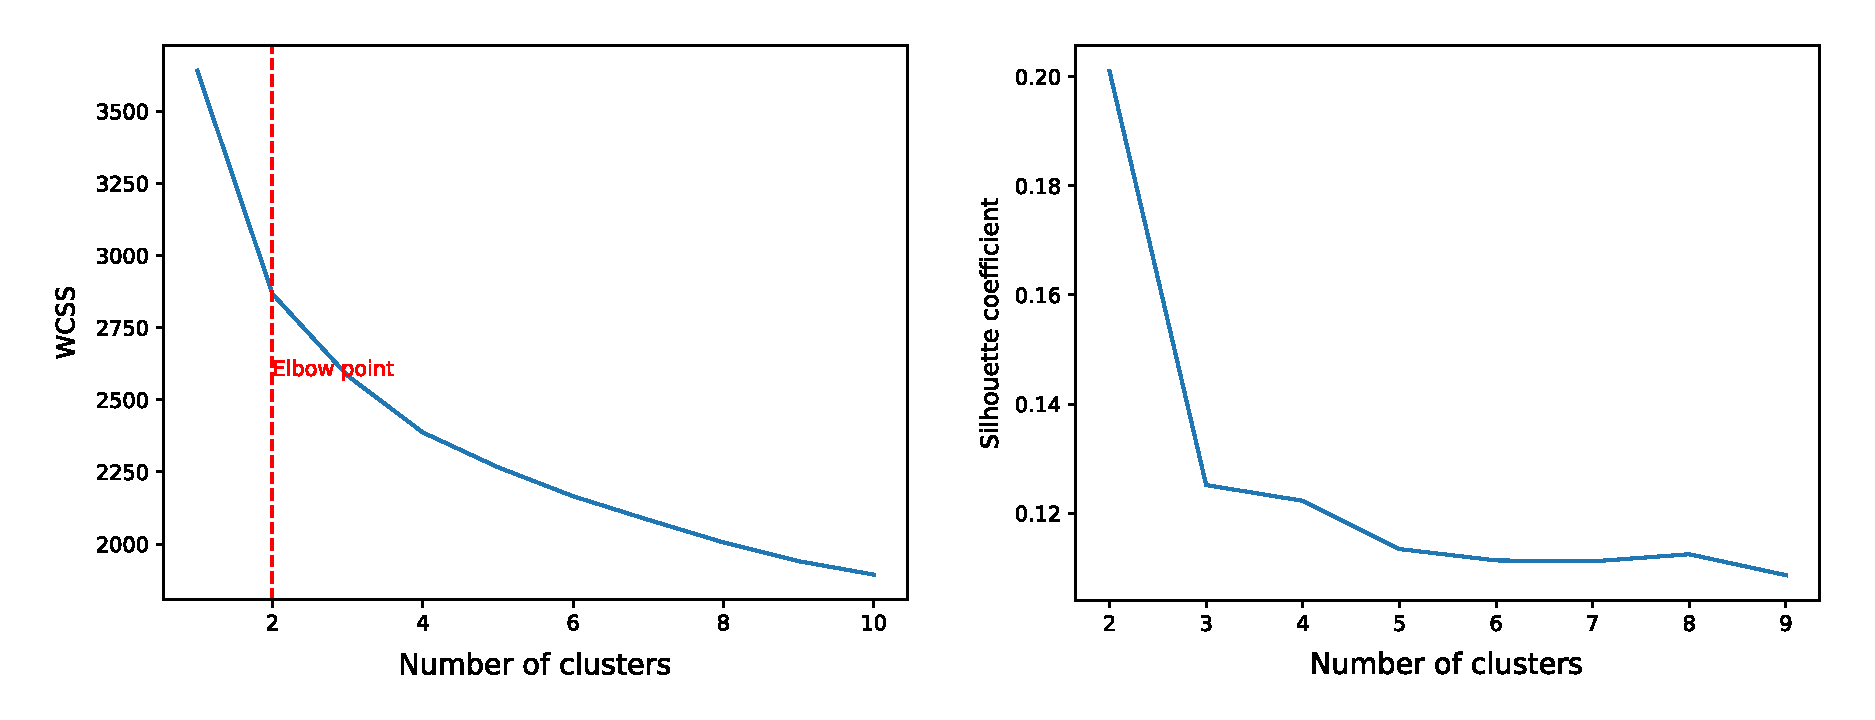
\includegraphics[width = \textwidth]{figs/elbow+silhouette_plot.pdf}
  \caption{Elbow and Silhouette plot to determine the optimal number of clusters before applying PCA. WCSS stands for Within-Cluster Sum of Square.}
  \label{fig:elbow+silhouette}
\end{figure}

\begin{figure}[htb]
  \centering
  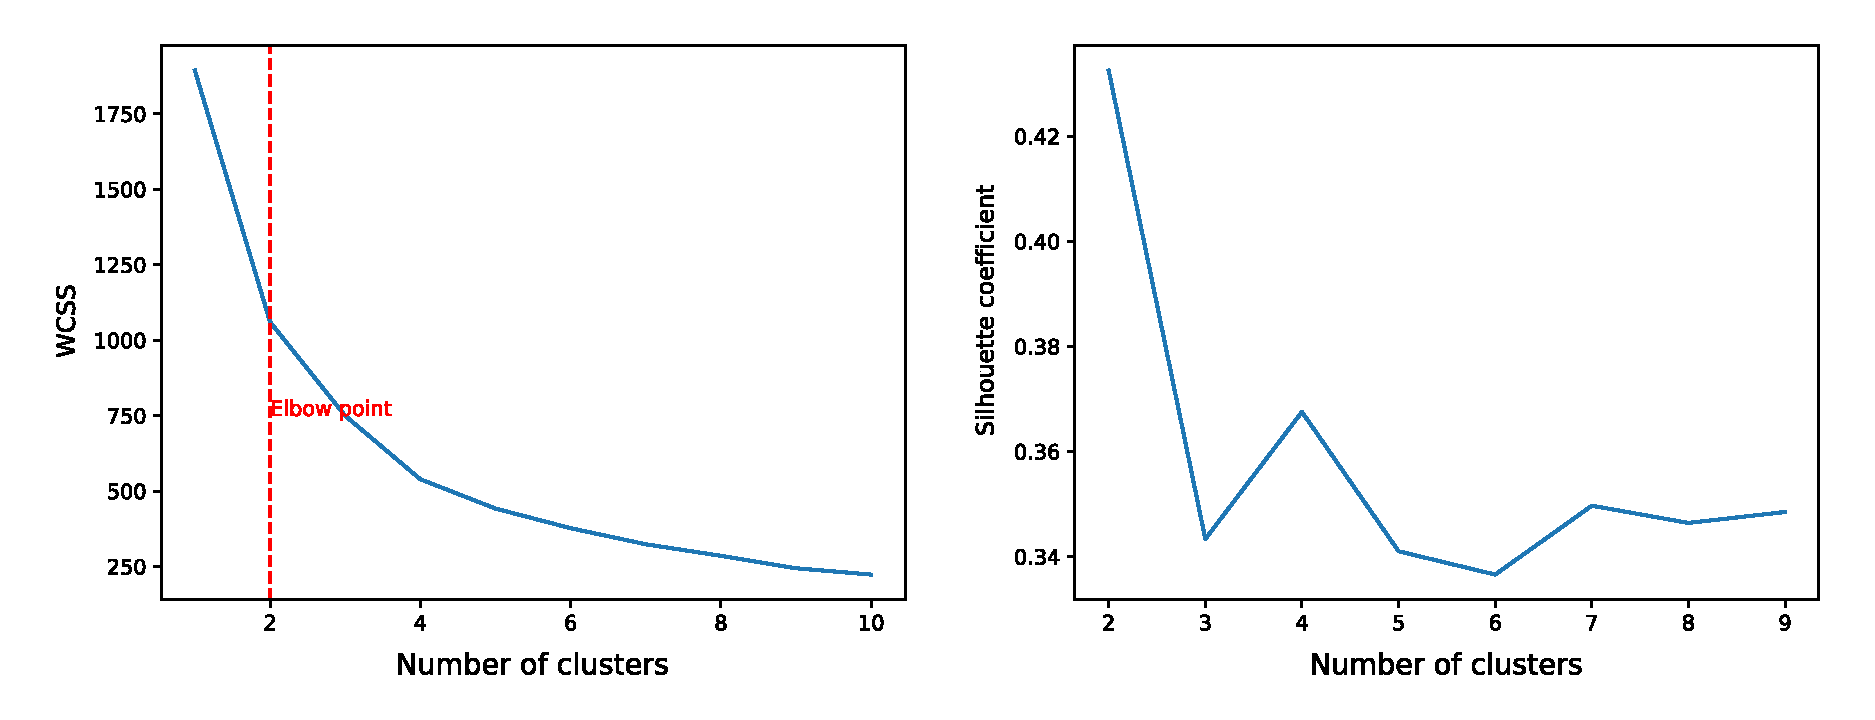
\includegraphics[width = \textwidth]{figs/elbow+silhouette_plot_PCA.pdf}
  \caption{Elbow and Silhouette plot to determine the optimal number of clusters after applying PCA. WCSS stands for Within-Cluster Sum of Square.}
  \label{fig:elbow+silhouette_PCA}
\end{figure}

\begin{table}[htb]
\caption{Comparison of results of evaluation metrics for K-Means clustering with and without PCA.}
\label{tab:K-Means_eval}
\begin{tabular*}{\linewidth}{@{\extracolsep{\fill}}lcc@{}}
\toprule
Metric  & \multicolumn{1}{l}{With PCA} & \multicolumn{1}{l}{Without PCA} \\ 
\midrule
Silhouette Coefficient $\uparrow$  & 0.43      & 0.21  \\
Calinski-Harabasz Index $\uparrow$ & 258.27    & 88.82 \\
Davies-Bouldin Index $\downarrow$    & 0.87      & 1.71  \\ 
\bottomrule
\end{tabular*}
\end{table}

We use evaluation metrics such as Calinski-Harabasz Index~\cite{harabasz1974dendrite} and Davies-Bouldin Index~\cite{davies1979cluster} to choose the one with best performance. The Calinski-Harabasz Index prioritizes tight, well-separated clusters, while the Davies-Bouldin Index penalizes clusters with high internal variation or proximity. Analyzing both helps identify the optimal cluster number (k) balancing compactness and separation in our data. In table~\ref{tab:K-Means_eval}, we can see that applying PCA gives us a comparatively better evaluation score. 

% \subsubsection{Results \& Findings}

% \begin{table}[htb]
% \caption{Comparison between cluster means between the clusters created with and without PCA. Here the factors are New Tech (NT), Impulsive Decision (ID), Too Busy To Cook (BC), Don't Like to Cook (DLC), Ordering is Easy (OE), Options to Choose (OC), Ordering is Inexpensive (OI), Promotional Offers and Discounts (POD), Quick Delivery (QD), Food Safety (FS), Food is Nutritious (FN).}
% \label{tab:k-means_results_both}
% \begin{tabular*}{\linewidth}{@{\extracolsep{\fill}}lcccc@{}}
% \toprule
% Factors               & \multicolumn{2}{c}{With PCA} & \multicolumn{2}{c}{Without PCA} \\ 
% \cmidrule(l){2-3} \cmidrule(l){4-5}
%                         & Cluster 0    & Cluster 1      & Cluster 0    & Cluster 1  \\ 
% \midrule    
% NT                & 1.45         & 2.47           & 1.45         & 2.48       \\
% ID     & 1.19         & 2.25           & 1.19         & 2.27       \\
% BC            & 1.47         & 2.31           & 1.47         & 2.34       \\
% DLC       & 1.08         & 2.04           & 1.08         & 2.04       \\
% OE          & 1.95         & 3.29           & 1.95         & 3.38       \\
% OC       & 1.75         & 3.35           & 1.75         & 3.44       \\
% OI    & 0.83         & 1.86           & 0.83         & 1.90       \\
% POD         & 1.53         & 2.92           & 1.53         & 3.02       \\
% QD         & 1.29         & 2.59           & 1.29         & 2.65       \\
% FS             & 1.17         & 1.98           & 1.17         & 2.02       \\
% FN            & 1.29         & 1.64           & 1.29         & 1.66       \\ 
% \bottomrule
% \end{tabular*}
% \end{table}

% On table~\ref{tab:k-means_results_both}, we have the mean values of each cluster. We show the values of both with PCA applied and without it.  On cluster 0 which contains respondents who tend to order less and cluster 1 represents the people who order comparatively more. We can see that people of cluster 0 find food delivered by OFO services to not be inexpensive with the mean value for 'Ordering Inexpensive' as 0.83 and 0.97. Whereas, people belonging in cluster 1 tend to find the food from the OFO services to lack nutritious values with mean value for 'Nutritious' as 1.64 and 1.66.

\section{Empirical Analysis}
Now, we use the 331 valid responses out of the 343 responses we receive, to show some statistical description of the dataset and do some exploratory data analysis:


% \begin{table}[htb]
%     \caption{Distribution of Gender.}
%     \label{tab:gender_distribution}
%     \begin{tabular*}{\linewidth}{@{\extracolsep{\fill}}lcc@{}}
%         \toprule
%         Gender            & Frequency & Percentage \\
%         \midrule
%         Male              & 202       & 61.03\%      \\
%         Female            & 125       & 37.76\%      \\
%         Prefer not to say & 4         & 1.21\%       \\
%         \bottomrule
%     \end{tabular*}
% \end{table}

\begin{minipage}{.5\textwidth}
\centering
  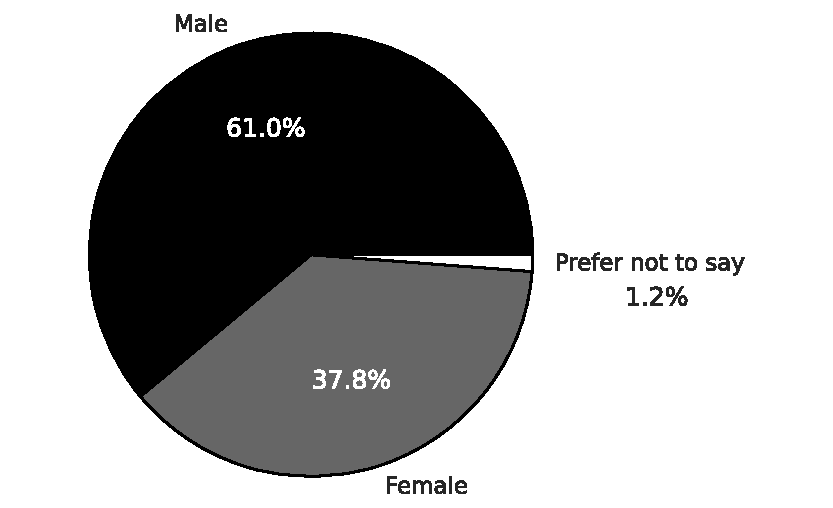
\includegraphics[width=.9\linewidth]{figs/gender_distribution.pdf}
  \captionof{figure}{Distribution of Gender.}
  \label{fig:gender_distribution}
\end{minipage}%
\begin{minipage}{.5\textwidth}
\centering
  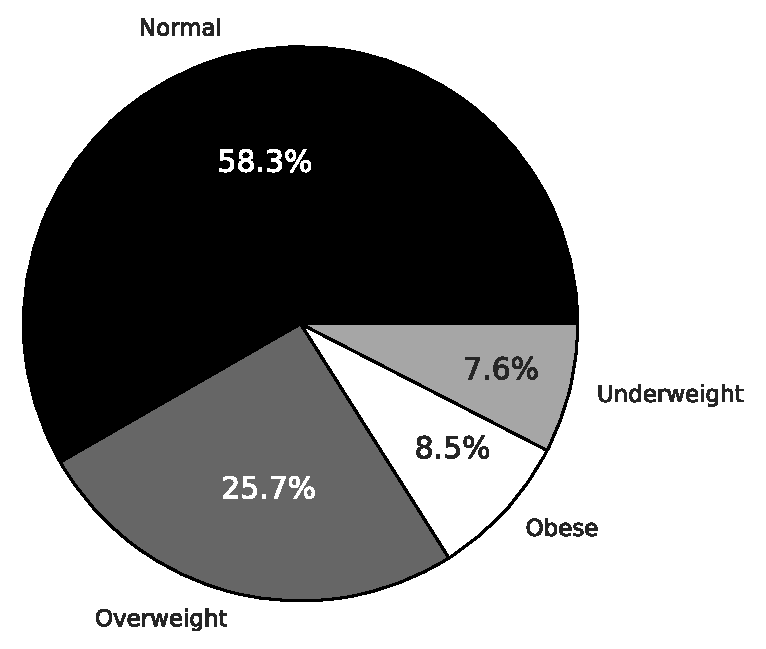
\includegraphics[width=.65\linewidth]{figs/bmi_distribution.pdf}
  \captionof{figure}{Distribution of BMI.}
  \label{fig:bmi_distribution}
\end{minipage}

According to figure \ref{fig:gender_distribution}, most of the participants are male (61.03\%). We have received 125 responses from female participants (37.76\%) and 4 participants preferred not to disclose their gender (1.21\%).

% \begin{table}[htb]
%     \caption{Distribution of BMI.}
%     \label{tab:bmi_distribution}
%     \begin{tabular*}{\linewidth}{@{\extracolsep{\fill}}lcc@{}}
%         \toprule
%         BMI & Frequency & Percentage \\
%         \midrule
%         Underweight & 25 & 7.6\% \\
%         Normal & 193 & 58.3\% \\
%         Overweight & 85 & 25.7\% \\
%         Obese & 28 & 8.5\%\\
%         \bottomrule
%     \end{tabular*}
% \end{table}

Analyzing the frequency distribution of BMI, it is evident that the majority of participants (58.3\%) fall into the category of normal BMI, with 193 calculated instances. The second-largest group (25.7\%) corresponds to participants with an overweight BMI, totalling 85 instances. Additionally, nearly 28 participants (8.5\%) have a BMI in the obese range. Furthermore, 25 participants (7.6\%) have a BMI indicating being underweight, as illustrated in Figure \ref{fig:bmi_distribution}.

\begin{figure}[htb]
  \centering
  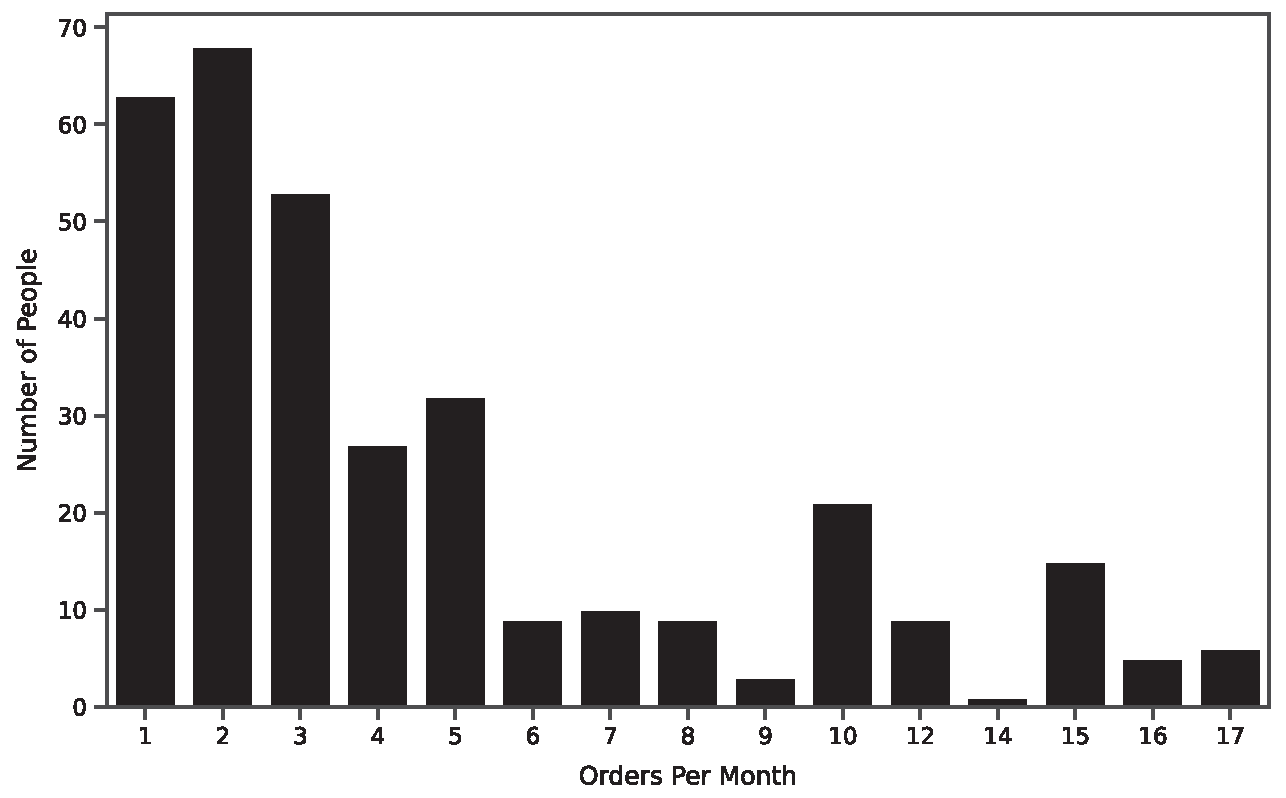
\includegraphics[width = \textwidth]{figs/order_frequency.pdf}
  \caption{Distribution of Online Food Orders Per Month.}
  \label{fig:orders_frequency}
\end{figure}

From Figure~\ref{fig:orders_frequency} we can see the number of foods ordered online per month by our survey participants. Here the range of ordering online is from 1 to 17. The highest number of ordering food in a month is 3 according to the chart. After that 2 and 1 are respectively the second and third highest numbers. 

% \begin{table}[htb]
%     \caption{Distribution of Educational Qualification.}
%     \label{tab:education}
%     \begin{tabular*}{\linewidth}{@{\extracolsep{\fill}}lcc@{}}
%         \toprule
%         Education & Frequency & Percentage \\
%         \midrule
%         Undergraduate & 252 & 76.13\% \\
%         High School & 22 & 6.65\% \\
%         Graduate/Post-Graduate/Phd & 57 & 17.22\% \\
%         \bottomrule
%     \end{tabular*}
% \end{table}

\begin{minipage}{.5\textwidth}
\centering
  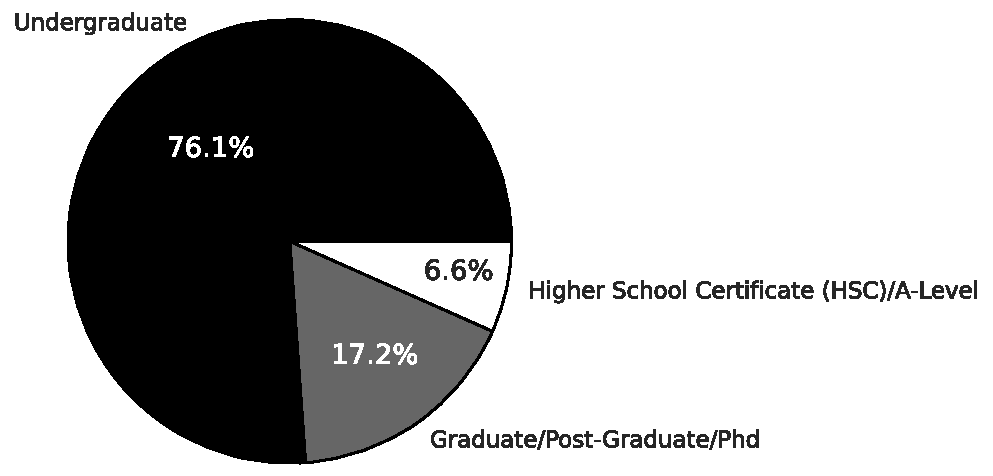
\includegraphics[width=.9\linewidth]{figs/educational_qualification.pdf}
  \captionof{figure}{Distribution of Educational Qualification.}
  \label{fig:education}
\end{minipage}%
\begin{minipage}{.5\textwidth}
\centering
  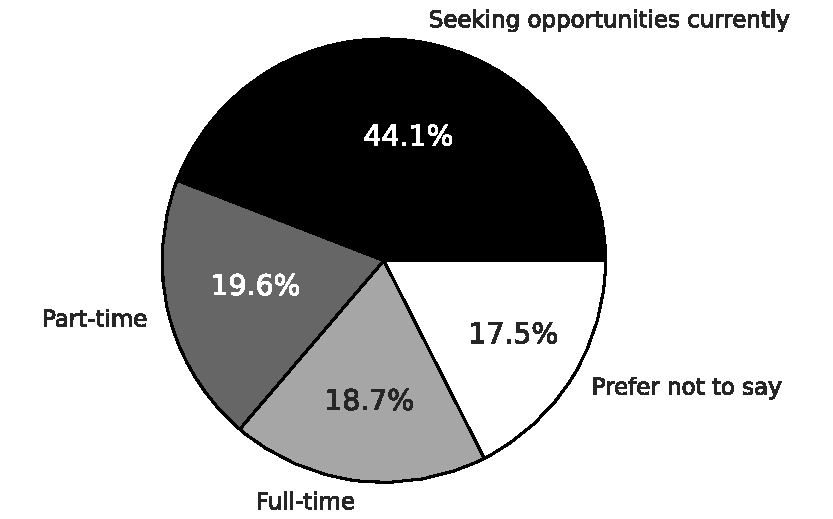
\includegraphics[width=.7\linewidth]{figs/employment_status.pdf}
  \captionof{figure}{Employment Status.}
  \label{fig:employment}
\end{minipage}

Figure~\ref{fig:education} shows that our online food ordering survey participants were mostly undergraduate students (76.13\%), with 252 responses. We also had 57 responses (17.22\%) from Graduate / Post-Graduate / Ph.D. students. The fewest responses (6.65\%) came from high school students, with only 22 responses.

% \begin{table}[htb]
%     \caption{Distribution of Employment Status.}
%     \label{tab:employment}
%     \begin{tabular*}{\linewidth}{@{\extracolsep{\fill}}lcc@{}}
%         \toprule
%         Employment Status & Frequency & Percentage \\
%         \midrule
%         Seeking opportunities currently  & 146 & 44.11\% \\
%         Part-time & 65 & 19.64\% \\
%         Full-time & 62 & 18.73\% \\
%         Prefer not to say & 58 & 17.52\% \\
%         \bottomrule
%     \end{tabular*}
% \end{table}

From Figure~\ref{fig:employment}, we see that 146 participants (44.11\%) are seeking career opportunities, while 62 participants (18.73\%) are full-time employed. A significant number of participants (58, or 17.52\%) did not mention their employment status. Furthermore, 65 participants (19.64\%) are doing part-time jobs.

% \begin{table}[htb]
%     \caption{Distribution of Financial Dependency.}
%     \label{tab:financial}
%     \begin{tabular*}{\linewidth}{@{\extracolsep{\fill}}lcc@{}}
%         \toprule
%         Financial Dependency & Frequency & Percentage \\
%         \midrule
%         Fully Dependent & 142 & 42.90\% \\
%         Partially Dependent & 136 & 41.09\% \\
%         Independent & 53 & 16.01\% \\
%         \bottomrule
%     \end{tabular*}
% \end{table}

\begin{minipage}{.5\textwidth}
\centering
  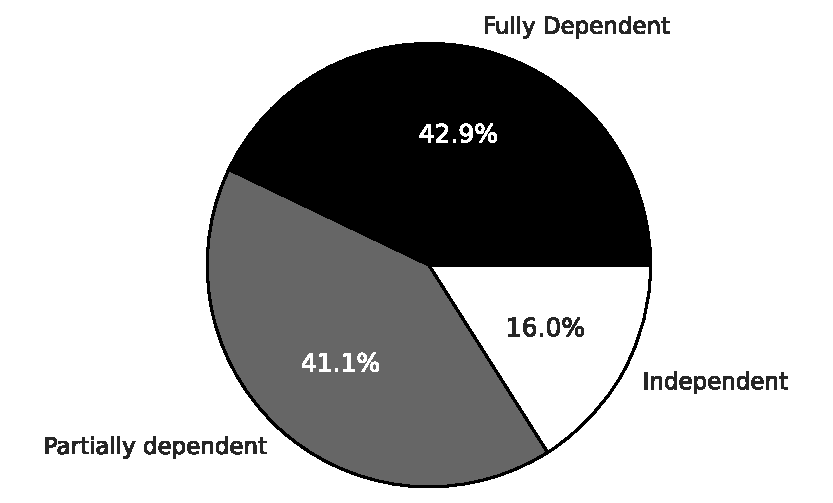
\includegraphics[width=.9\linewidth]{figs/financial_dependency.pdf}
  \captionof{figure}{Distribution of Financial Dependency.}
  \label{fig:financial}
\end{minipage}%
\begin{minipage}{.5\textwidth}
\centering
  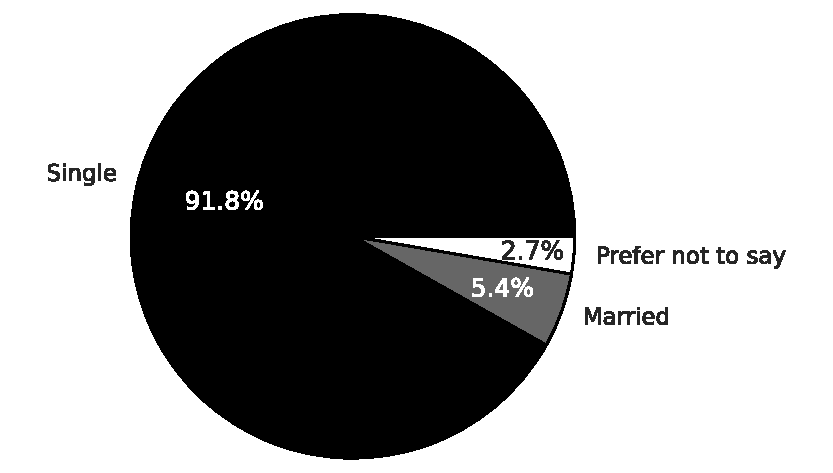
\includegraphics[width=.9\linewidth]{figs/marital_status.pdf}
  \captionof{figure}{Marital Status.}
  \label{fig:marital}
\end{minipage}


Inspecting the figure~\ref{fig:financial}, we see that 142 participants are fully dependent (42.90\%). The number of partially dependent (41.09\%) participants is 136. Lastly, 53 people responded to their status as independent (16.01\%). 

% \begin{table}[htb]
%     \caption{Distribution of Marital Status.}
%     \label{tab:marital}
%     \begin{tabular*}{\linewidth}{@{\extracolsep{\fill}}lcc@{}}
%         \toprule
%         Marital Status & Frequency & Percentage \\
%         \midrule
%         Single & 304 & 91.84\% \\
%         Married & 18 & 5.44\% \\
%         Prefer not to say & 9 & 2.72\% \\
%         \bottomrule
%     \end{tabular*}
% \end{table}


In figure~\ref{fig:marital}, we can see that 304 individuals are single (91. 84\%). We also have 18 participants who are married (5.44\%) and only 9 respondents did not mention their marital status (2.72\%). 

\begin{figure}[htb]
  \centering
  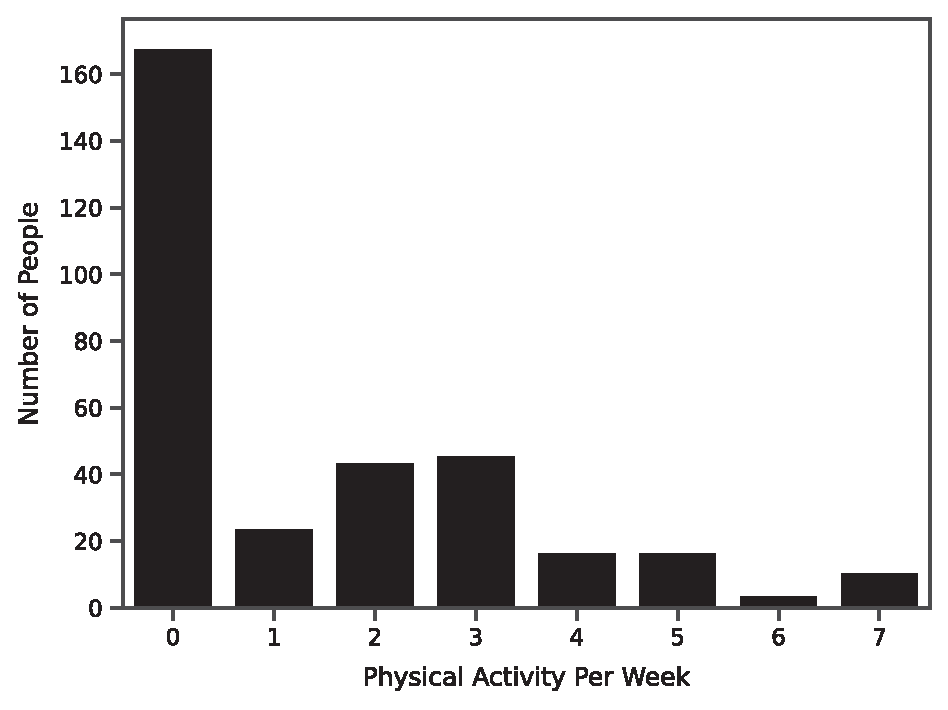
\includegraphics[width = \textwidth]{figs/physical_activity.pdf}
  \caption{Distribution of Physical Activity.}
  \label{fig:phy_act}
\end{figure}

Figure~\ref{fig:phy_act} shows the distribution of respondents' physical activity over a week. Over 160 participants reported not doing any physical activity, while fewer than 60 engaged in it 2 to 3 times per week. Only 20 or fewer reported doing it 4 to 7 times per week, and less than 40 did it once.

% \begin{table}[htb]
    % \caption{Distribution of Online Food Ordering History.}
    % \label{tab:ofo_history}
%     \begin{tabular*}{\linewidth}{@{\extracolsep{\fill}}lcc@{}}
%         \toprule
%         Ordering History & Frequency & Percentage \\
%         \midrule
%         Less than 3 months & 43 & 12.99\% \\
%         3-6 months & 21 & 6.34\% \\
%         More than 6 months & 262 & 80.66\% \\
%         \bottomrule
%     \end{tabular*}
% \end{table}

\begin{minipage}{.5\textwidth}
\centering
  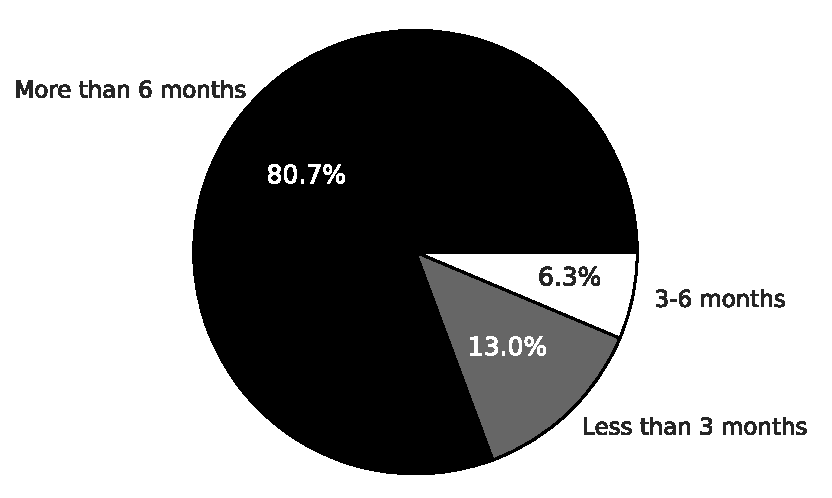
\includegraphics[width=.9\linewidth]{figs/ordering_history.pdf}
  \captionof{figure}{Distribution of OFO History.}
  \label{fig:ofo_history}
\end{minipage}%
\begin{minipage}{.5\textwidth}
\centering
  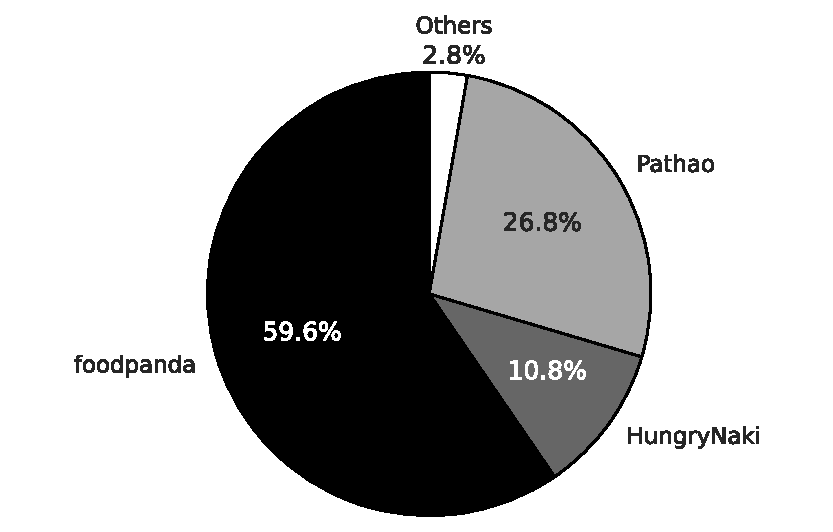
\includegraphics[width=.9\linewidth]{figs/ofo_apps.pdf}
  \captionof{figure}{Distribution of OFO Apps.}
  \label{fig:ofo_apps}
\end{minipage}

In figure~\ref{fig:ofo_history}, we can see that 262 participants have been using OFO services for more than 6 months (80.66\%). Moreover, we can notice that 43 participants have used it for less than 3 months (12.99\%). Furthermore, 21 participants have been using it for 3 to 6 months (6.34\%).

% \begin{table}[htb]
    % \caption{Distribution of the Use of Online Food Ordering Apps.}
    % \label{tab:ofo_apps}
%     \begin{tabular*}{\linewidth}{@{\extracolsep{\fill}}lcc@{}}
%         \toprule
%         OFO Apps & Frequency & Percentage \\
%         \midrule
%         foodpanda & 302 & 59.57\% \\
%         HungryNaki & 55 & 10.85\% \\
%         Pathao & 136 & 26.82\% \\
%         Others & 14 & 2.76\% \\
%         \bottomrule
%     \end{tabular*}
% \end{table}

Most of the survey participants (59.57\%) are using foodpanda and the number is 302. The second highest (26.82\%) used app by our survey participants is Pathao where the number of users is 136. Thirdly, 55 people are using Hungrynaki (10.85\%). Lastly, we can see that 14 survey participants are using other apps (2.76\%). 

% \begin{table}[htb]
    % \caption{Distribution of Online Food Ordering Time.}
    % \label{tab:ordering_time}
%     \begin{tabular*}{\linewidth}{@{\extracolsep{\fill}}lcc@{}}
%         \toprule
%         Ordering Time & Frequency & Percentage \\
%         \midrule
%         Breakfast & 17 & 2.86\% \\
%         Lunch & 138 & 23.23\% \\
%         Evening Snacks & 227 & 38.22\% \\
%         Dinner & 176 & 29.63\% \\
%         Midnight Snacks & 36 & 6.06\% \\
%         \bottomrule
%     \end{tabular*}
% \end{table}

\begin{figure}[htb]
  \centering
  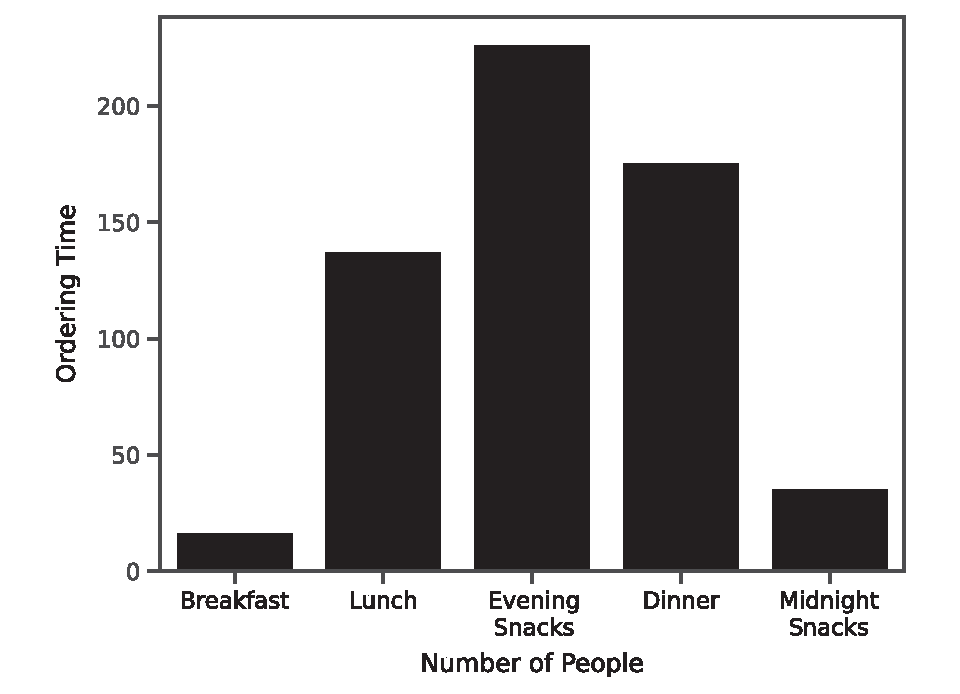
\includegraphics[width = \textwidth]{figs/ordering_time_bar.pdf}
    \caption{Distribution of Online Food Ordering Time.}
    \label{fig:ordering_time}
\end{figure}

Figure~\ref{fig:ordering_time} gives us an idea of when people tend to order food. Firstly, most of the participants (38.22\%) are ordering food for evening snacks and the number is 227. Secondly, 176 participants voted for online food ordering time as dinner (29.63\%). Thirdly, 138 people responded to lunchtime for ordering food online (23.23\%). Moreover, The number of ordering food online for midnight snacks (6.06\%) is 36. Furthermore, 17 people selected breakfast for ordering food online (2.86\%).

\begin{figure}[htb]
  \centering
  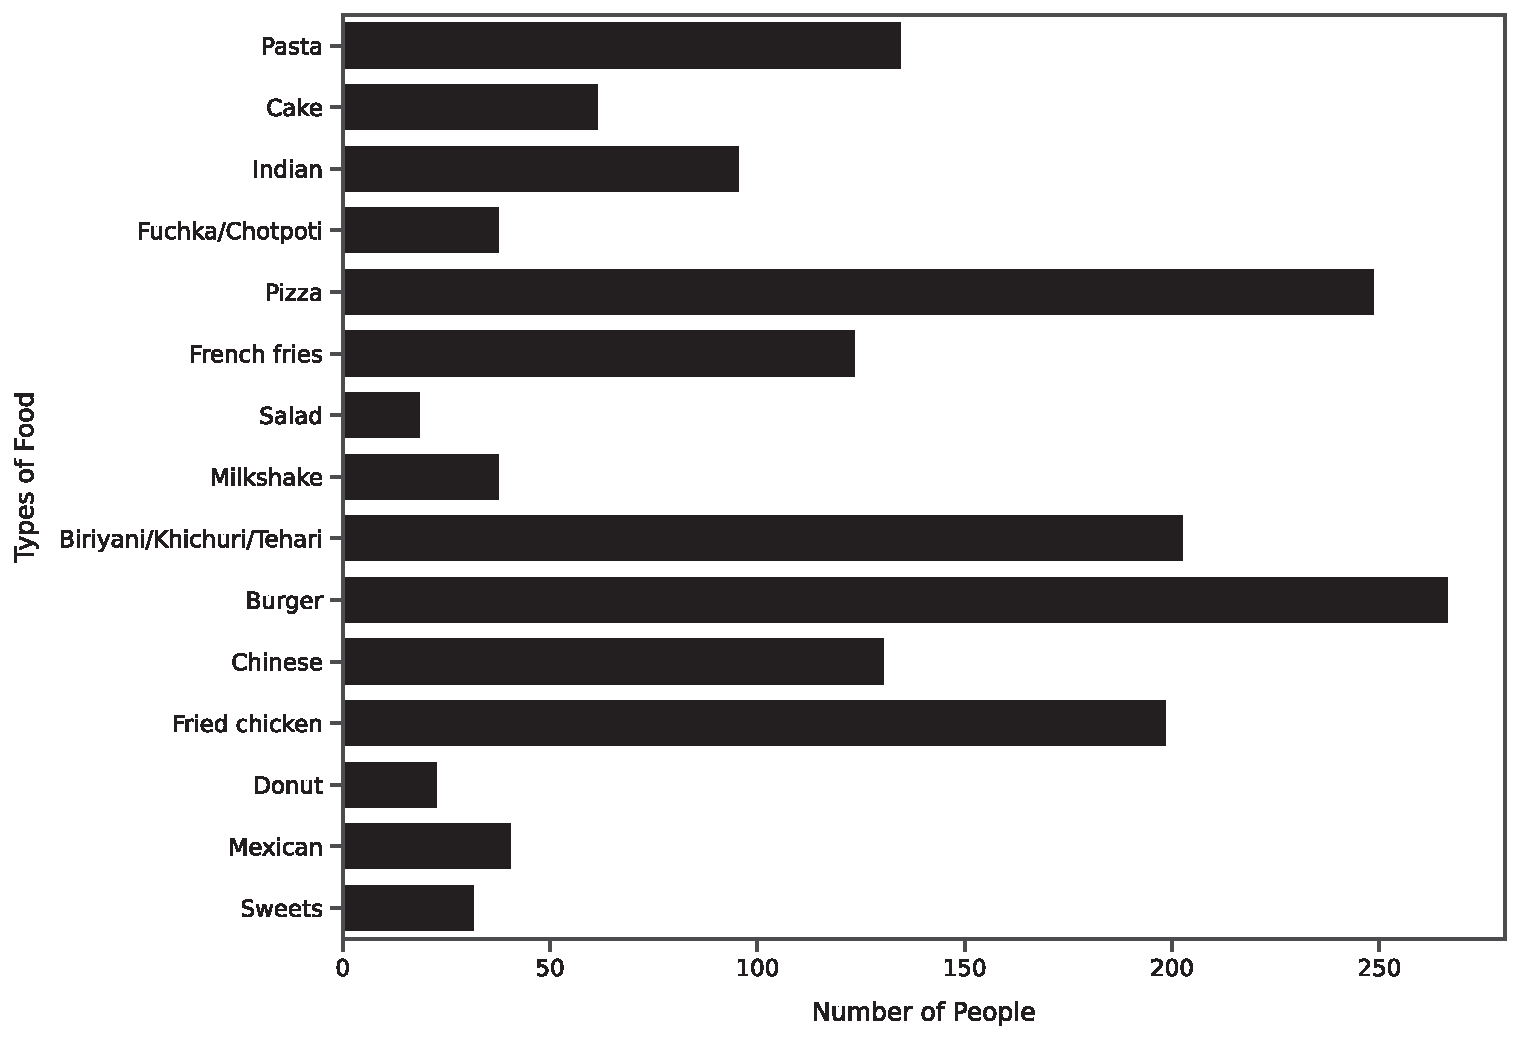
\includegraphics[width = \textwidth]{figs/food_distribution.pdf}
  \caption{Distribution of type of foods ordered through online platforms.}
  \label{fig:food_distribution}
\end{figure}

From figure~\ref{fig:food_distribution}, we can see that the majority tend to order burgers (267) and pizzas (249) when ordering food online, which consist of high amounts of saturated fat and salt. Salads (19) are among the lowest to be ordered. There were some food types with only one entry, we dropped those since those are negligible.

\begin{figure}[htb]
  \centering
  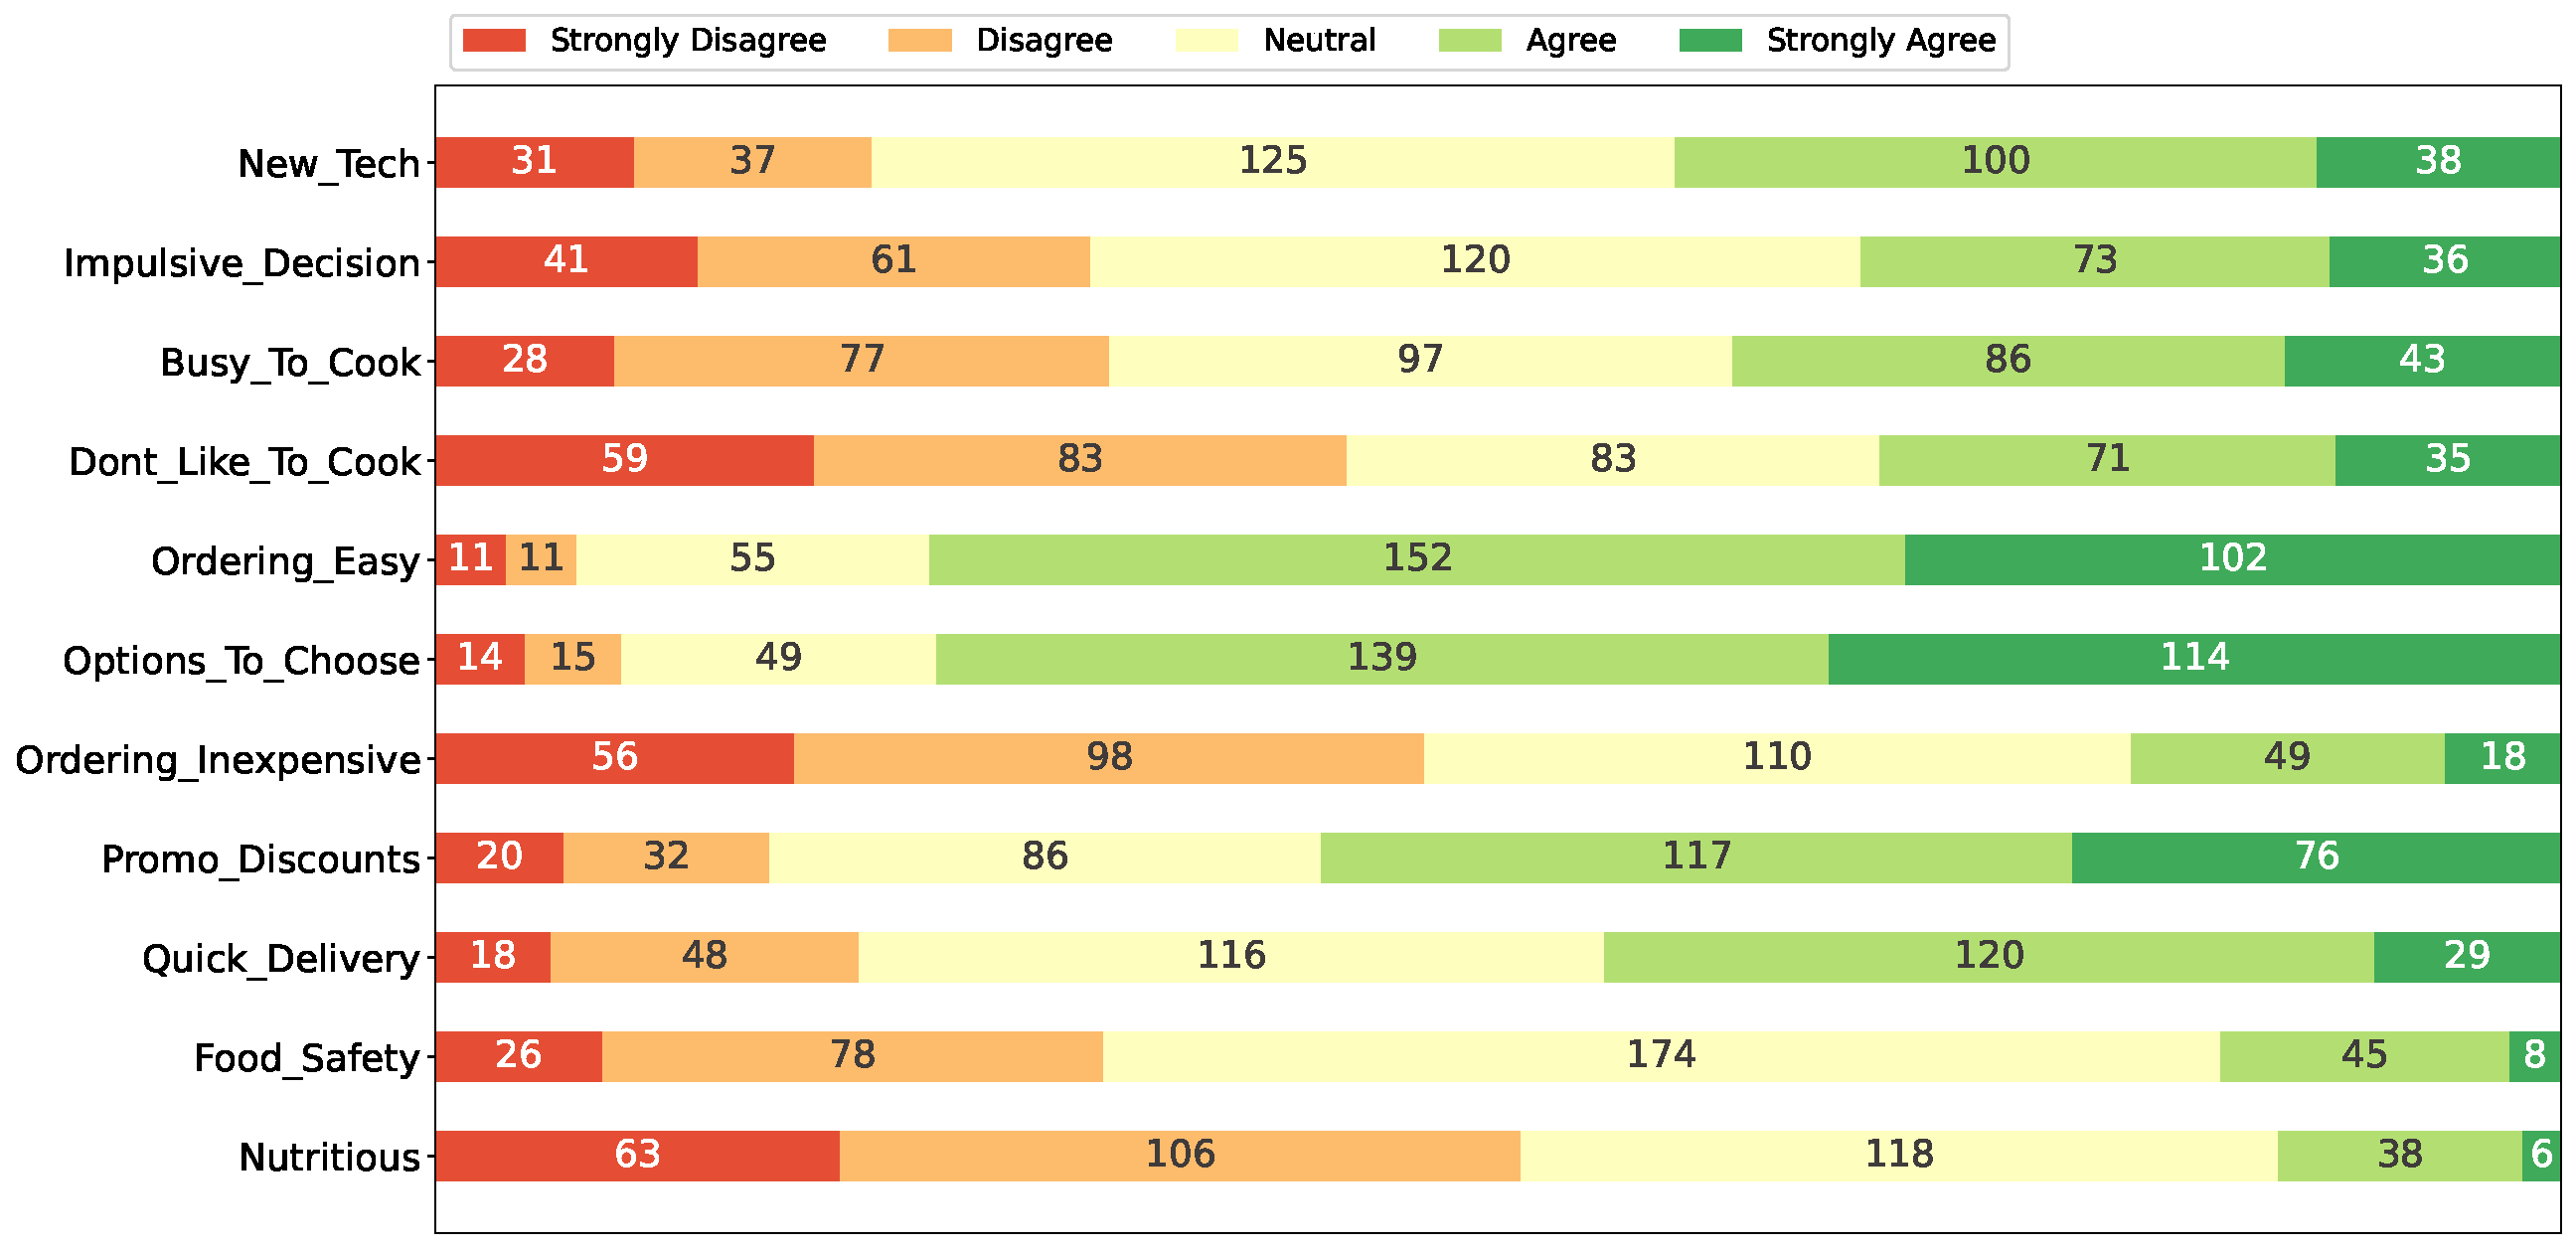
\includegraphics[width = \textwidth]{figs/likert.pdf}
  \caption{Distribution of Factors that Influence Online Food Orders.}
  \label{fig:factors}
\end{figure}

The figure~\ref{fig:factors} gives us an idea of the importance of each factor on a Likert scale. Firstly, we found that 100 people agreed and 125 responded as neutral to being inclined to try out new technologies. Secondly, 120 people voted neutral and 73 agreed to make impulsive decisions to order food online. Thirdly, 97 people responded neutral, 86 agreed and 77 disagreed with being too busy to cook food themselves and leaning towards OFO services. There is a match with 83 numbers of responses where each is allocated for disagree and neutral where the factor is people don't like to cook. A huge number of participants agreed that ordering food online is easy, where 152 people agreed and 102 strongly agreed. Again, lots of people agreed that they like having a variety of options to choose their desired food from OFO platforms, where 139 people agreed and 114 strongly agreed. In the case of choosing to order food online due to being inexpensive, 110 participants responded as neutral and 98 people disagreed. 117 people agreed that promotional discounts convince them to order food online whereas 86 responded to neutral. A big portion of our survey participants agreed that ordering food online allows them to get their food quickly and the response number is 120, besides 116 people voted neutral. 174 of the participants stayed neutral when they were asked if they think their food is safe and hygienic and 78 participants disagreed with it. Lastly, very few survey participants believe that their online food ordered item is nutritious with 118 people responding as neutral, 106 disagreed and 63 participants strongly disagreed with the factor.

\section{Results}

\subsection{Results of Most Influential Factors Mining}
The results of the experiments which are done to find the most influencing factors are shown in table~\ref{tab:factors_results} gives us an idea of which factors influence a person to use OFO services. 

\begin{table}[htb]
\caption{Influential Factors in Online Food Orders: Comparing Mean, Standard Deviation, OLS, Decision Tree, and Random Forest Values.}
\label{tab:factors_results}
\begin{tabular*}{\linewidth}{@{\extracolsep{\fill}}lccccc@{}}
\hline
    Factors & Mean & SD & OLS & DT & RF \\
    \hline
    New Tech & 2.23 & 1.09 & 0.39 & 0.01 & 0.22 \\
    Impulsive Decision & 2.01 & 1.16 & 0.90 & 0.34 & 0.22 \\
    Busy To Cook & 2.12 & 1.16 & 0.18 & 0.05 & 0.10 \\
    Don't Like To Cook & 1.82 & 1.25 & 0.33 & 0.01 & 0.13 \\
    Ordering Easy & 2.98 & 0.95 & 0.65 & 0.11 & 0.08 \\
    Options To Choose & 2.98 & 1.03 & 0.15 & 0.01 & 0.06 \\
    Ordering Inexpensive & 1.62 & 1.10 & 0.27 & 0.22 & 0.07 \\
    Promo Discounts & 2.60 & 1.12 & 0.33 & 0.01 & 0.09 \\
    Quick Delivery & 2.28 & 1.00 & 0.11 & 0.01 & 0.05 \\
    Food Safety & 1.79 & 0.86 & -0.40 & 0.01 & 0.05 \\
    Nutritious & 1.45 & 0.98 & -0.32 & 0.28 & 0.09 \\
    \hline
\end{tabular*}
\end{table}

The mean values based on solely the responses from the respondents suggest that the most important factors in influencing people's decision to order food online are the convenience of ordering (mean score of 2.98), the variety of options available (mean score of 2.98), and promotional offers and discounts (mean score of 2.60).

\subsection{Results of Hypothesis Testing}
The results of the hypothesis study point out that the first hypothesis, H1 is accepted and the null hypothesis is rejected as the p-value is $<$ 0.001, which is less than ($\alpha$ = 0.05). This means that people who tend to try out new technologies also feel that ordering food online is convenient and easy. 

For the second hypothesis, H2 is rejected as the p-value (0.1143) is higher than the $\alpha$ (0.05). This means we could not find any significant relationship between being too busy to cook and making impulsive decisions when ordering food online. 

The third hypothesis, H3 is accepted and the null hypothesis is rejected as the p-value ($<$ 0.001) is lower than the $\alpha$ (0.05). This means there is a significant relationship between having many options to choose from when ordering food online and not liking to cook. 

The fourth hypothesis, H4 is accepted and the null hypothesis is rejected as the p-value ($<$ 0.001) is less than the $\alpha$ (0.05). This means that there exists a significant relationship between finding ordering food online to be inexpensive and using promo codes and discounts when ordering food online. 

\subsection{Results of Correlation Analysis}
The results from Pearson correlation and Spearman's rank correlation which was done between BMI and orders per month, give us a p-value of $2.43^{-7}$ and $0.003$ respectively, which suggests that there exists a statistically significant positive correlation between the two variables since both these values are less than 0.05. The coefficient values are $0.28$ and $0.15$ respectively which suggests there exists a weak positive correlation and a very weak positive correlation~\cite{jaadi_2019}. 


\begin{table}[htb]
    \caption{Results of Point-biserial Correlation on BMI vs Orders Per Month.}
    \label{tab:Pbi_BMI_OPM}
    \begin{tabular*}{\linewidth}{@{\extracolsep{\fill}}lccl@{}}
        \toprule
        BMI & P-value & Coefficient & Relationship \\
        \midrule
        Underweight & 0.84 & -0.01 & Rejected \\
        Normal & $1.97^{-5}$ & -0.23 &  Weak Negative \\
        Overweight & 0.04 & 0.04 & Very Weak Positive \\
        Obese & $1.13^{-10}$ & 0.34 & Weak Positive \\
        \bottomrule
    \end{tabular*}
\end{table}


The results shown in table~\ref{tab:Pbi_BMI_OPM} suggest that due to insufficient p-value, any relation between Underweight and orders per month is rejected, normal weight has a weak negative relationship, overweight has a very weak positive relationship and obese has a weak positive relationship. 


\begin{table}[htb]
    \caption{Results of Correlation analysis between physical activity and orders per month.}
    \label{tab:pearson_spearman_phy_OPM}
    \begin{tabular*}{\linewidth}{@{\extracolsep{\fill}}lccl@{}}
        \toprule
        Test & P-value & Coefficient & Relationship \\
        \midrule
        Pearson & 0.026 & -0.12 & Very Weak Negative \\
        Spearman & 0.085 & -0.10 & Rejected \\
        \bottomrule
    \end{tabular*}
\end{table}


As seen in table~\ref{tab:pearson_spearman_phy_OPM}, we can see that there exists a very weak negative relation between physical activity and orders per month which suggests that people who tend to order more may exercise less. However, the results from Spearman's test are rejected as the p-value is 0.085, which is greater than the $\alpha$ value of 0.05.


\begin{table}[htb]
    \caption{Results of Point-biserial Correlation on Ordering History and Orders Per Month.}
    \label{tab:Pbi_OH_OPM}
    \begin{tabular*}{\linewidth}{@{\extracolsep{\fill}}lccl@{}}
        \toprule
        Ordering History & P-value & Coefficient & Relationship \\
        \midrule
        < 3 months & $1.40^{-5}$ & -0.23 & Weak Negative \\
        3 - 6 months & 0.66 & 0.02 &  Rejected \\
        > 6 months & $<$ 0.0001 & 0.18 & Very Weak Positive \\
        \bottomrule
    \end{tabular*}
\end{table}


The results of correlation analysis between ordering history and orders per month as seen on table~\ref{tab:Pbi_OH_OPM} show that people who have been using OFO for more than 6 months tend to order more. The coefficient value of -0.23 suggests that there exists a weak relationship between ordering frequency and people who have been using this type of service for less than 3 months. However, due to the p-value (0.66) being higher than the $\alpha$ value of 0.05, any relationship between people who have been ordering for 3-6 months is rejected. 

\subsection{Results of the Prediction of Frequent Users of OFO services}
The results of the prediction model can be seen in table~\ref{tab:pred_before}.

\begin{table}[htb]
    \caption{Comparison of results among prediction models before feature selection.}
    % \caption{Comparison of results among prediction models}
    \label{tab:pred_before}
    \begin{tabular*}{\linewidth}{@{\extracolsep{\fill}}lcccc@{}}
        \toprule
        Model & Accuracy & Precision & Recall & F1-Score \\
        \midrule
        LR  & 0.78 & 0.65 & 0.57 & 0.58 \\
        NB  & 0.66 & 0.54 & 0.54 & 0.53 \\
        DT  & 0.59 & 0.46 & 0.46 & 0.46 \\
        RF  & 0.79 & 0.73 & 0.56 & 0.55 \\
        GBM & 0.71 & 0.51 & 0.50 & 0.50 \\
        KNN & 0.80 & 0.72 & 0.64 & 0.66 \\
        \bottomrule
    \end{tabular*}
\end{table}


We can see that out of 6 models, Random Forest performs the best with 81\% accuracy. In comparison, Naive Bayes performed worst with 68\% accuracy. Random Forest also has the best precision score of 0.74 which means it has a high level of precision in identifying positive instances. Additionally, Random Forest correctly identified 64\% of the positive instances as seen in the Recall column.

\begin{table}[htb]
    \caption{Comparison of results among prediction models after feature selection.}
    \label{tab:pred_after}
    \begin{tabular*}{\linewidth}{@{\extracolsep{\fill}}lcccc@{}}
        \toprule
        Model & Accuracy & Precision & Recall & F1-Score \\
        \midrule
        LR  & 0.78 & 0.64 & 0.55 & 0.54 \\
        NB  & 0.79 & 0.70 & 0.58 & 0.59 \\
        DT  & 0.68 & 0.55 & 0.56 & 0.56 \\
        RF  & 0.81 & 0.74 & 0.61 & 0.63 \\
        GBM & 0.76 & 0.61 & 0.56 & 0.56 \\
        KNN & 0.74 & 0.56 & 0.53 & 0.52 \\
        \bottomrule
    \end{tabular*}
\end{table}

\subsection{Results of Customer Segmentation}
\begin{table}[htb]
\caption{Comparison between cluster means between the clusters created with and without PCA. Here the factors are New Tech (NT), Impulsive Decision (ID), Too Busy To Cook (BC), Don't Like to Cook (DLC), Ordering is Easy (OE), Options to Choose (OC), Ordering is Inexpensive (OI), Promotional Offers and Discounts (POD), Quick Delivery (QD), Food Safety (FS), Food is Nutritious (FN).}
\label{tab:k-means_results_both}
\begin{tabular*}{\linewidth}{@{\extracolsep{\fill}}lcccc@{}}
\toprule
Factors               & \multicolumn{2}{c}{With PCA} & \multicolumn{2}{c}{Without PCA} \\ 
\cmidrule(l){2-3} \cmidrule(l){4-5}
                        & Cluster 0    & Cluster 1      & Cluster 0    & Cluster 1  \\ 
\midrule    
NT                & 1.45         & 2.47           & 1.45         & 2.48       \\
ID     & 1.19         & 2.25           & 1.19         & 2.27       \\
BC            & 1.47         & 2.31           & 1.47         & 2.34       \\
DLC       & 1.08         & 2.04           & 1.08         & 2.04       \\
OE          & 1.95         & 3.29           & 1.95         & 3.38       \\
OC       & 1.75         & 3.35           & 1.75         & 3.44       \\
OI    & 0.83         & 1.86           & 0.83         & 1.90       \\
POD         & 1.53         & 2.92           & 1.53         & 3.02       \\
QD         & 1.29         & 2.59           & 1.29         & 2.65       \\
FS             & 1.17         & 1.98           & 1.17         & 2.02       \\
FN            & 1.29         & 1.64           & 1.29         & 1.66       \\ 
\bottomrule
\end{tabular*}
\end{table}

In table~\ref{tab:k-means_results_both}, we have the mean values of each cluster. We show the values of both with PCA applied and without it.  Cluster 0 contains respondents who tend to order less and Cluster 1 represents the people who order comparatively more. We can see that people of cluster 0 find food delivered by OFO services to not be inexpensive with the mean value for 'Ordering Inexpensive' as 0.83 and 0.97. Whereas, people belonging to cluster 1 tend to find the food from the OFO services to lack nutritious values with the mean value for 'Nutritious' as 1.64 and 1.66.

\section{Discussions}

The results of OLS show that the most influencing factors are making impulsive decisions (coefficient value of 0.90), and convenience of ordering (coefficient value of 0.65). On the other hand, food safety (coefficient value of -0.40) and nutritious value of the food (coefficient value of -0.36) have a negative impact. The results of the most influential factor mining support some of the findings from previous works. The high coefficient value on impulsive decision supports~\cite{alagoz_2012} as they also find that hedonic motivation is one of the important factors. The positive impact of ease of convenience as found by~\cite{kale_customer_perception_2020, alagoz_2012, vinish2021} is supported by our results as well. We find that food safety is a major concern as it has a negative impact when using OFO services, this is also supported by~\cite{hong_2021}.

Additionally, we can see that the results of the hypothesis testing show that hypotheses, H1, H2 and H3 were accepted and H2 were rejected. This suggests some of the factors are not necessarily independent of each other.

The results of the Pearson Correlation suggest that when we treat BMI as a continuous value, there exists a weak positive correlation between BMI and orders per month. When treating BMI as a categorical value, the results of the Spearman Correlation show that there exists a weak positive correlation. Although, this does not indicate that there is necessarily any causation here. Moreover, when we treat the BMI values as binary categories it shows that there exists a very weak positive and a weak positive correlation for overweight and obese respectively. This supports the research conducted by Dana ~\etal~\cite{dana2021}. However, people with normal BMIs show a weak negative relationship with orders of food per month. So, even though there exists a positive relationship between being overweight or obese and ordering a lot of food per month, it is however very weak. These findings can be used in future studies to combine with other factors to see if any causality exists.

We can see in table~\ref{tab:pred_after}, that after applying feature selection the performance of Naive Bayes, Decision Tree, Random Forest and Gradient Boosting Machine improves. Although the performance of the KNN decreases and that of Logistic Regression stays the same as before. This can also be seen in figure~\ref{fig:compare_pred}.

\begin{figure}[htb]
  \centering
  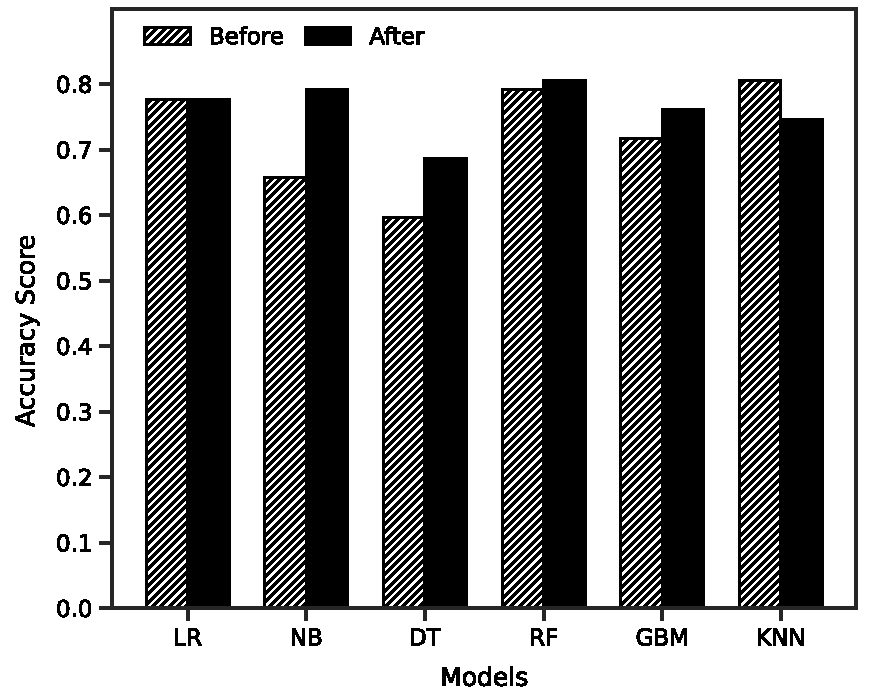
\includegraphics[width = \textwidth]{figs/accuracy_plot.pdf}
  \caption{Comparison between results of prediction models before and after applying feature selection.}
  \label{fig:compare_pred}
\end{figure}

Moreover, the results of customer segmentation show that respondents in both clusters show the tendency to order food because it is convenient, there are a variety of options to choose from, and due to the availability of promotional offers and discounts. However, we can see that people of cluster 0 find food delivered by OFO services to not be inexpensive. Whereas, people belonging to cluster 1 tend to find the food from the OFO services to lack nutritious values.

\section{Conclusion}

% This research investigates the factors that influence customers to use online food ordering platforms in the context of Bangladesh. We created a dataset containing the activities of OFO service users, which is non-existent, especially in the Bangladeshi context. Our findings reveal that there exists a weak positive correlation between BMI and orders per month. Furthermore, it shows that people who tend to order more, happen to have higher BMI. However, it is important to note that a correlation does not necessarily imply causation. We find that making impulsive decisions, the convenience of ordering and the availability of promotional offers and discounts are the most important factors behind the frequency of ordering food online. Additionally, we achieve a 81\% accuracy in classifying frequent users of OFO services. This study contributes to a nuanced understanding of the dynamics driving online food consumption behavior in the Bangladeshi context.

This research delves into the determinants influencing the utilization of online food ordering (OFO) platforms on a global scale, with a specific focus on the context of Bangladesh. We have generated a unique dataset capturing the behaviours of OFO service users, a noteworthy contribution considering the limited existing data, particularly within the Bangladeshi context. Our findings unveil a subtle positive correlation between Body Mass Index (BMI) and monthly order frequencies, suggesting that individuals with higher BMIs tend to place orders more frequently. It is crucial to highlight that correlation does not imply causation. The study identifies impulsive decision-making, ordering convenience, and the allure of promotional offers and discounts as pivotal factors driving the frequency of online food ordering. Furthermore, we achieve an 81\% accuracy in classifying frequent users of OFO services. This research extends beyond regional boundaries, considering a densely populated country Bangladesh as a Test-case scenario, offering insights into the nuanced dynamics that shape online food consumption behavior on a global scale.

%\subsection{Limitations \& Future Work}
%Our research has its limitations. First of all, our data was collected from people of ages 16-30, which means that it may not accurately reflect the characteristics and perspectives of the entire population. Moreover, our study was cross-sectional, which means that we cannot make causal inferences from our results. Future research could be done with even bigger data with more factors to consider. Another research opportunity is to include more factors such as advertisements, spending level to get better insights.

\section*{Dataset availability and usage policy}
% The data underpinning the findings of this study are accessible from the corresponding author upon reasonable request. The datasets employed and/or scrutinized during the course of the current study have been deposited in both the Mendeley data repository and IEEE dataport. This ensures transparency and facilitates the reproducibility of our research, allowing fellow researchers and interested parties to validate and build upon our findings. We encourage collaboration and further exploration of the dataset for the advancement of knowledge within the scientific community.

The data underpinning the findings of this study are accessible from the corresponding author upon reasonable request.

\section*{Funding:}
This research did not receive any specific grant from funding agencies in the public, commercial, or not-for-profit sectors.

% \section{Installation}

% The package is available at author resources page at Elsevier
% (\url{http://www.elsevier.com/locate/latex}).
% The class may be moved or copied to a place, usually,\linebreak
% \verb+$TEXMF/tex/latex/elsevier/+, %$%%%%%%%%%%%%%%%%%%%%%%%%%%%%
% or a folder which will be read                   
% by \LaTeX{} during document compilation.  The \TeX{} file
% database needs updation after moving/copying class file.  Usually,
% we use commands like \verb+mktexlsr+ or \verb+texhash+ depending
% upon the distribution and operating system.

% \section{Front matter}

% The author names and affiliations could be formatted in two ways:
% \begin{enumerate}[(1)]
% \item Group the authors per affiliation.
% \item Use footnotes to indicate the affiliations.
% \end{enumerate}
% See the front matter of this document for examples. 
% You are recommended to conform your choice to the journal you 
% are submitting to.

% \section{Bibliography styles}

% There are various bibliography styles available. You can select the
% style of your choice in the preamble of this document. These styles are
% Elsevier styles based on standard styles like Harvard and Vancouver.
% Please use Bib\TeX\ to generate your bibliography and include DOIs
% whenever available.

% Here are two sample references: \cite{Fortunato2010}
% \cite{Fortunato2010,NewmanGirvan2004}
% \cite{Fortunato2010,Vehlowetal2013}

% \section{Floats}
% {Figures} may be included using the command,\linebreak 
% \verb+\includegraphics+ in
% combination with or without its several options to further control
% graphic. \verb+\includegraphics+ is provided by {graphic[s,x].sty}
% which is part of any standard \LaTeX{} distribution.
% {graphicx.sty} is loaded by default. \LaTeX{} accepts figures in
% the postscript format while pdf\LaTeX{} accepts {*.pdf},
% {*.mps} (metapost), {*.jpg} and {*.png} formats. 
% pdf\LaTeX{} does not accept graphic files in the postscript format. 

% \begin{figure}
% 	\centering
% 		\includegraphics[scale=.75]{figs/Fig1.pdf}
% 	\caption{The evanescent light - $1S$ quadrupole coupling
% 	($g_{1,l}$) scaled to the bulk exciton-photon coupling
% 	($g_{1,2}$). The size parameter $kr_{0}$ is denoted as $x$ and
% 	the \PMS is placed directly on the cuprous oxide sample ($\delta
% 	r=0$, See also Table \protect\ref{tbl1}).}
% 	\label{FIG:1}
% \end{figure}


% The \verb+table+ environment is handy for marking up tabular
% material. If users want to use {multirow.sty},
% {array.sty}, etc., to fine control/enhance the tables, they
% are welcome to load any package of their choice and
% {cas-sc.cls} will work in combination with all loaded
% packages.

% \begin{table}[width=.9\linewidth,cols=4,pos=h]
% \caption{This is a test caption. This is a test caption. This is a test
% caption. This is a test caption.}\label{tbl1}
% \begin{tabular*}{\tblwidth}{@{} LLLL@{} }
% \toprule
% Col 1 & Col 2 & Col 3 & Col4\\
% \midrule
% 12345 & 12345 & 123 & 12345 \\
% 12345 & 12345 & 123 & 12345 \\
% 12345 & 12345 & 123 & 12345 \\
% 12345 & 12345 & 123 & 12345 \\
% 12345 & 12345 & 123 & 12345 \\
% \bottomrule
% \end{tabular*}
% \end{table}

% \section[Theorem and ...]{Theorem and theorem like environments}

% {cas-sc.cls} provides a few shortcuts to format theorems and
% theorem-like environments with ease. In all commands the options that
% are used with the \verb+\newtheorem+ command will work exactly in the same
% manner. {cas-sc.cls} provides three commands to format theorem or
% theorem-like environments: 

% \begin{verbatim}
%  \newtheorem{theorem}{Theorem}
%  \newtheorem{lemma}[theorem]{Lemma}
%  \newdefinition{rmk}{Remark}
%  \newproof{pf}{Proof}
%  \newproof{pot}{Proof of Theorem \ref{thm2}}
% \end{verbatim}


% The \verb+\newtheorem+ command formats a
% theorem in \LaTeX's default style with italicized font, bold font
% for theorem heading and theorem number at the right hand side of the
% theorem heading.  It also optionally accepts an argument which
% will be printed as an extra heading in parentheses. 

% \begin{verbatim}
%   \begin{theorem} 
%    For system (8), consensus can be achieved with 
%    $\|T_{\omega z}$ ...
%      \begin{eqnarray}\label{10}
%      ....
%      \end{eqnarray}
%   \end{theorem}
% \end{verbatim}  


% \newtheorem{theorem}{Theorem}

% \begin{theorem}
% For system (8), consensus can be achieved with 
% $\|T_{\omega z}$ ...
% \begin{eqnarray}\label{10}
% ....
% \end{eqnarray}
% \end{theorem}

% The \verb+\newdefinition+ command is the same in
% all respects as its \verb+\newtheorem+ counterpart except that
% the font shape is roman instead of italic.  Both
% \verb+\newdefinition+ and \verb+\newtheorem+ commands
% automatically define counters for the environments defined.

% The \verb+\newproof+ command defines proof environments with
% upright font shape.  No counters are defined. 


% \section[Enumerated ...]{Enumerated and Itemized Lists}
% {cas-sc.cls} provides an extended list processing macros
% which makes the usage a bit more user friendly than the default
% \LaTeX{} list macros.   With an optional argument to the
% \verb+\begin{enumerate}+ command, you can change the list counter
% type and its attributes.

% \begin{verbatim}
%  \begin{enumerate}[1.]
%  \item The enumerate environment starts with an optional
%    argument `1.', so that the item counter will be suffixed
%    by a period.
%  \item You can use `a)' for alphabetical counter and '(i)' 
%   for roman counter.
%   \begin{enumerate}[a)]
%     \item Another level of list with alphabetical counter.
%     \item One more item before we start another.
%     \item One more item before we start another.
%     \item One more item before we start another.
%     \item One more item before we start another.
% \end{verbatim}

% Further, the enhanced list environment allows one to prefix a
% string like `step' to all the item numbers.  

% \begin{verbatim}
%  \begin{enumerate}[Step 1.]
%   \item This is the first step of the example list.
%   \item Obviously this is the second step.
%   \item The final step to wind up this example.
%  \end{enumerate}
% \end{verbatim}

% \section{Cross-references}
% In electronic publications, articles may be internally
% hyperlinked. Hyperlinks are generated from proper
% cross-references in the article.  For example, the words
% \textcolor{black!80}{Fig.~1} will never be more than simple text,
% whereas the proper cross-reference \verb+\ref{tiger}+ may be
% turned into a hyperlink to the figure itself:
% \textcolor{blue}{Fig.~1}.  In the same way,
% the words \textcolor{blue}{Ref.~[1]} will fail to turn into a
% hyperlink; the proper cross-reference is \verb+\cite{Knuth96}+.
% Cross-referencing is possible in \LaTeX{} for sections,
% subsections, formulae, figures, tables, and literature
% references.

% \section{Bibliography}

% Two bibliographic style files (\verb+*.bst+) are provided ---
% {model1-num-names.bst} and {model2-names.bst} --- the first one can be
% used for the numbered scheme. This can also be used for the numbered
% with new options of {natbib.sty}. The second one is for the author year
% scheme. When  you use model2-names.bst, the citation commands will be
% like \verb+\citep+,  \verb+\citet+, \verb+\citealt+ etc. However when
% you use model1-num-names.bst, you may use only \verb+\cite+ command.

% \verb+thebibliography+ environment.  Each reference is a\linebreak
% \verb+\bibitem+ and each \verb+\bibitem+ is identified by a label,
% by which it can be cited in the text:

% \noindent In connection with cross-referencing and
% possible future hyperlinking it is not a good idea to collect
% more that one literature item in one \verb+\bibitem+.  The
% so-called Harvard or author-year style of referencing is enabled
% by the \LaTeX{} package {natbib}. With this package the
% literature can be cited as follows:

% \begin{enumerate}[\textbullet]
% \item Parenthetical: \verb+\citep{WB96}+ produces (Wettig \& Brown, 1996).
% \item Textual: \verb+\citet{ESG96}+ produces Elson et al. (1996).
% \item An affix and part of a reference:\break
% \verb+\citep[e.g.][Ch. 2]{Gea97}+ produces (e.g. Governato et
% al., 1997, Ch. 2).
% \end{enumerate}

% In the numbered scheme of citation, \verb+\cite{<label>}+ is used,
% since \verb+\citep+ or \verb+\citet+ has no relevance in the numbered
% scheme.  {natbib} package is loaded by {cas-sc} with
% \verb+numbers+ as default option.  You can change this to author-year
% or harvard scheme by adding option \verb+authoryear+ in the class
% loading command.  If you want to use more options of the {natbib}
% package, you can do so with the \verb+\biboptions+ command.  For
% details of various options of the {natbib} package, please take a
% look at the {natbib} documentation, which is part of any standard
% \LaTeX{} installation.

% \appendix
% \section{My Appendix}
% Appendix sections are coded under \verb+\appendix+.

% \verb+\printcredits+ command is used after appendix sections to list 
% author credit taxonomy contribution roles tagged using \verb+\credit+ 
% in frontmatter.
\printcredits

% \clearpage
%% Loading bibliography style file
\bibliographystyle{model1-num-names}
% \bibliographystyle{cas-model2-names}

% Loading bibliography database
\bibliography{cas-refs}


%\vskip3pt

%\bio{figs/iftekhar_mobin.jpg}
%Dr. Md Iftekharul Mobin, (Member, IEEE), Assistant Professor of Faculty of Science and Technology at American International University-Bangladesh (AIUB). Dr. Mobin's scholarly pursuits are anchored in a diverse range of research domains, including Natural Language Processing (NLP), time-series prediction, health informatics, Internet of Things (IoT), and Image processing. Earned his Ph.D. from Queen Mary University of London. He achieved Queen Mary scholarship and the ImpactQM scholarship, in acknowledgment of his contributions to industry-academia partnerships. Dr. Mobin's research endeavors have received support from Bangladesh's Ministry of Information and Communication Technology (ICT). He served as a software engineer in the United Kingdom, Japan, and Bangladesh for several years. This dual exposure to both academic and industry settings has enriched his perspectives and insights of industry academia collaboration and implications. He has served as a program committee member of international conferences, editor, and reviewer for various conferences and journals worldwide. 
%\endbio

% \bio{figs/pic1}
% Author biography with author photo.
% Author biography. Author biography. Author biography.
% Author biography. Author biography. Author biography.
% Author biography. Author biography. Author biography.
% Author biography. Author biography. Author biography.
% Author biography. Author biography. Author biography.
% Author biography. Author biography. Author biography.
% Author biography. Author biography. Author biography.
% Author biography. Author biography. Author biography.
% Author biography. Author biography. Author biography.
% \endbio

% \bio{figs/pic1}
% Author biography with author photo.
% Author biography. Author biography. Author biography.
% Author biography. Author biography. Author biography.
% Author biography. Author biography. Author biography.
% Author biography. Author biography. Author biography.
% \endbio

\end{document}

